\documentclass[spanish, a3paper,twoside]{xc_project_a3}
\usepackage[spanish]{babel}
\usepackage[T1]{fontenc}
\usepackage[utf8]{inputenc}
\usepackage{boldline}
\usepackage[hidelinks]{hyperref}
\usepackage{colortbl}
\usepackage{amsmath}
\usepackage{pdfpages}
\usepackage{caption}[=v1]
\usepackage{flafter}
\usepackage{enumitem} %% compact description lists.
\usepackage{wrapfig} %% Wrapping text around figures.
\usepackage{longtable}
\usepackage{multicol}
\usepackage{nonfloat}
\usepackage{multirow}
\usepackage{wasysym}
\usepackage{gensymb}
\usepackage{xtab,booktabs}

\renewcommand{\titProy}{\footnotesize{Proyecto}}
\renewcommand{\titDoc}{Documento}
\title{\underline{\textbf{\titDoc}}}
\author{XC ingeniería estructural, S.L.}
\date{\today}
\renewcommand{\revision}{0.0}
%\portadilla
%\chapter*{\textbf{\titDoc}}
\minitoc

\newcommand{\ncols}{3}
\newcommand{\dir}{}
\setcounter{tocdepth}{5}

\begin{document}
\maketitle

\newpage
% Use Figure instead of figure for more than 2 columns of figures (multicols)
\newenvironment{Figure}
  {\par\medskip\noindent\minipage{\linewidth}}
  {\endminipage\par\medskip}
  
\twocolumn
 
\tableofcontents
\listoftables
\listoffigures
\newpage
\chapter{Introducción}
\section{Introducción}

%\onecolumn
%\begin{multicols}{\ncols}
\chapter{Datos y resultados del cálculo}\label{result_calc}
\section{Acciones}\label{fig_acciones}
\begin{figure}[ht]
\begin{center}
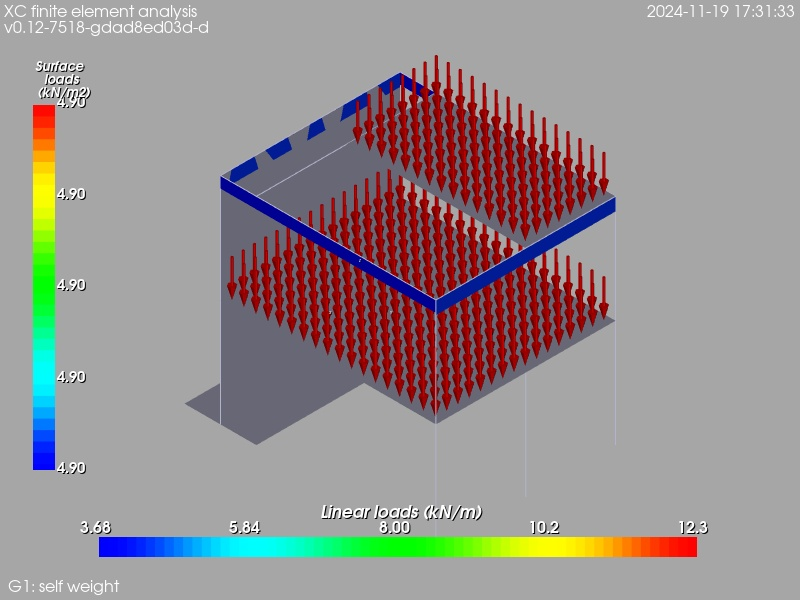
\includegraphics[width=\linewidth]{results/graphics/loads/GselfWeightoverallSet}
\caption{ G1: self weight, distribución de cargas.}
\label{GselfWeightoverallSet}
\end{center}
\end{figure}
\begin{figure}[ht]
\begin{center}
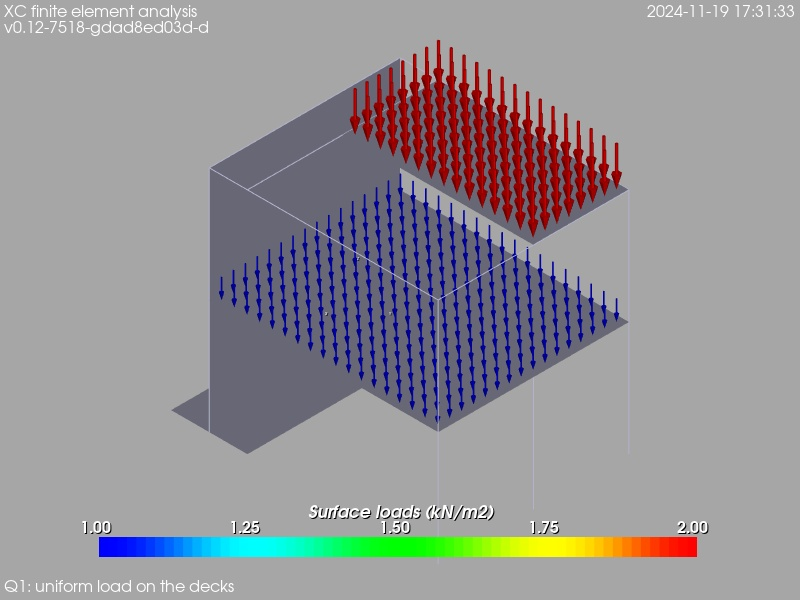
\includegraphics[width=\linewidth]{results/graphics/loads/QdecksoverallSet}
\caption{Q1: uniform load on the decks, distribución de cargas.}
\label{QdecksoverallSet}
\end{center}
\end{figure}
\begin{figure}[ht]
\begin{center}
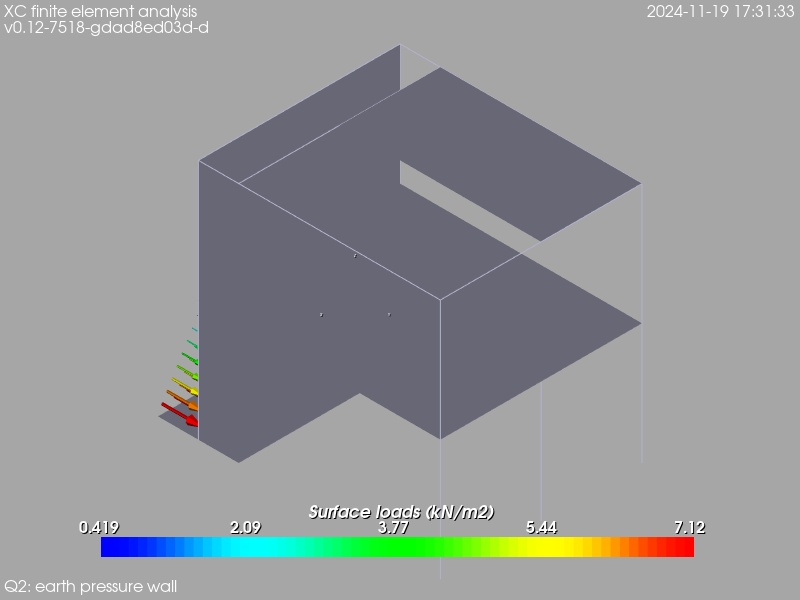
\includegraphics[width=\linewidth]{results/graphics/loads/QearthPressWalloverallSet}
\caption{Q2: earth pressure wall, distribución de cargas.}
\label{QearthPressWalloverallSet}
\end{center}
\end{figure}
\begin{figure}[ht]
\begin{center}
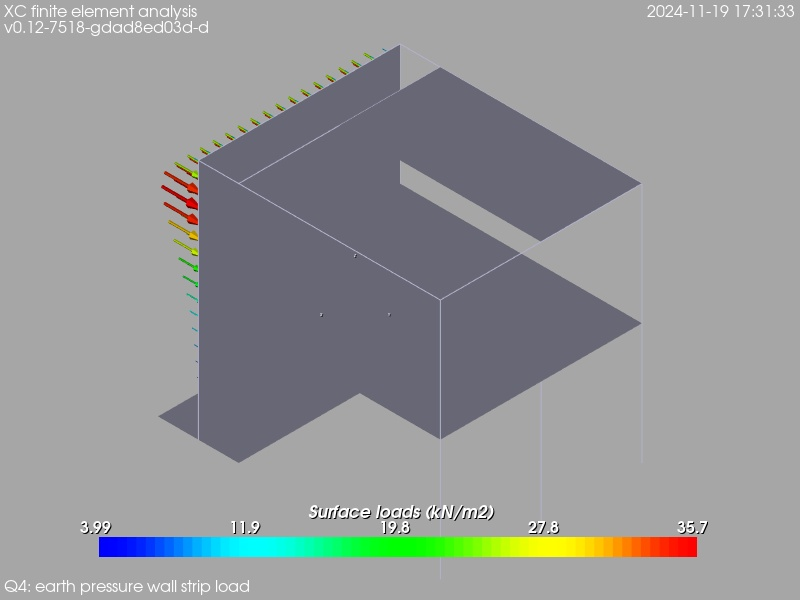
\includegraphics[width=\linewidth]{results/graphics/loads/QearthPWallStrLoverallSet}
\caption{Q4: earth pressure wall strip load, distribución de cargas.}
\label{QearthPWallStrLoverallSet}
\end{center}
\end{figure}
\begin{figure}[ht]
\begin{center}
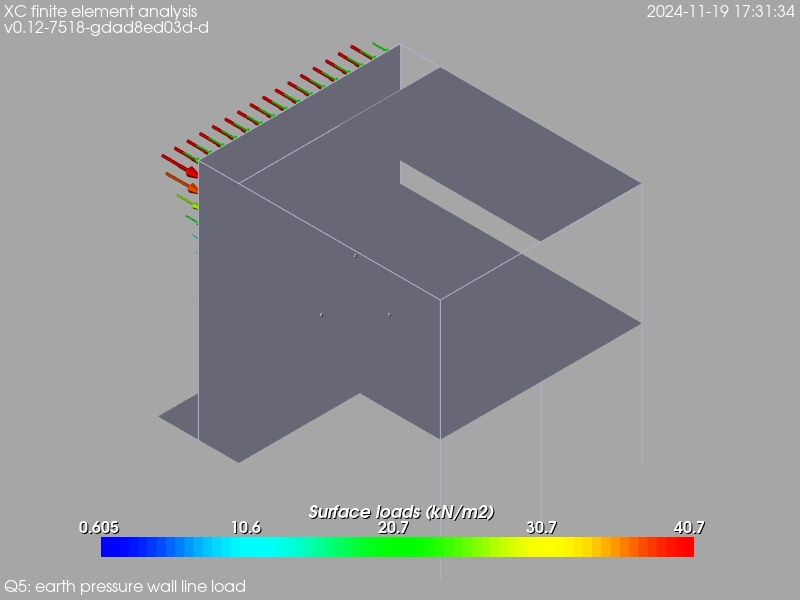
\includegraphics[width=\linewidth]{results/graphics/loads/QearthPWallLinLoverallSet}
\caption{Q5: earth pressure wall line load, distribución de cargas.}
\label{QearthPWallLinLoverallSet}
\end{center}
\end{figure}
\begin{figure}[ht]
\begin{center}
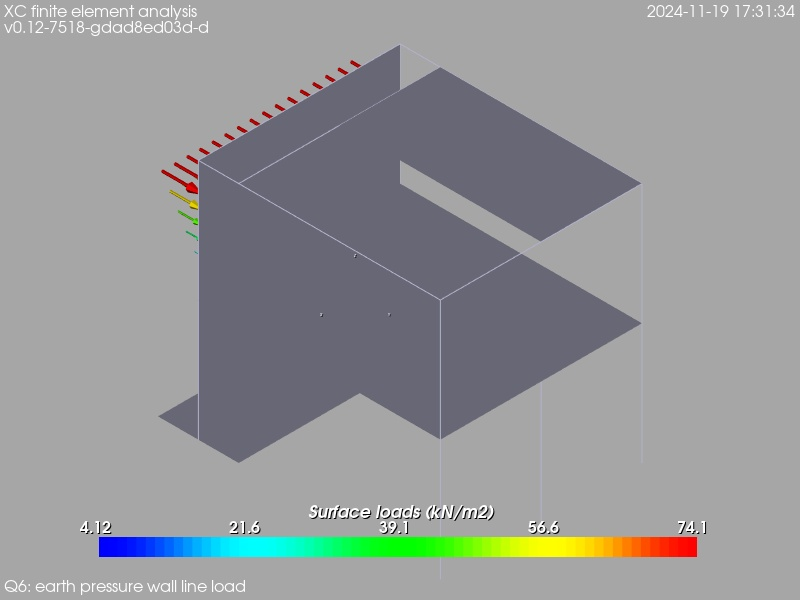
\includegraphics[width=\linewidth]{results/graphics/loads/QearthPWallHrzLoverallSet}
\caption{Q6: earth pressure wall line load, distribución de cargas.}
\label{QearthPWallHrzLoverallSet}
\end{center}
\end{figure}
\begin{figure}[ht]
\begin{center}
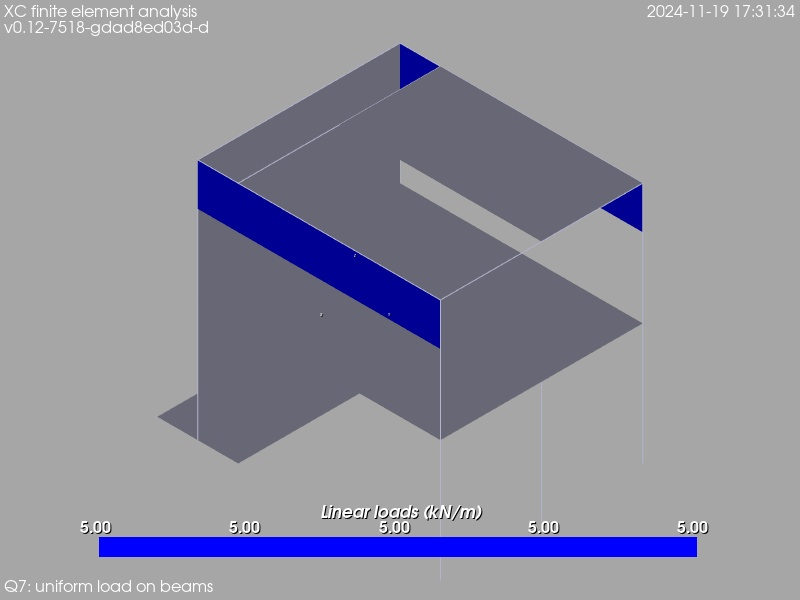
\includegraphics[width=\linewidth]{results/graphics/loads/qunifBeamsoverallSet}
\caption{Q7: uniform load on beams, distribución de cargas.}
\label{qunifBeamsoverallSet}
\end{center}
\end{figure}
\begin{figure}[ht]
\begin{center}
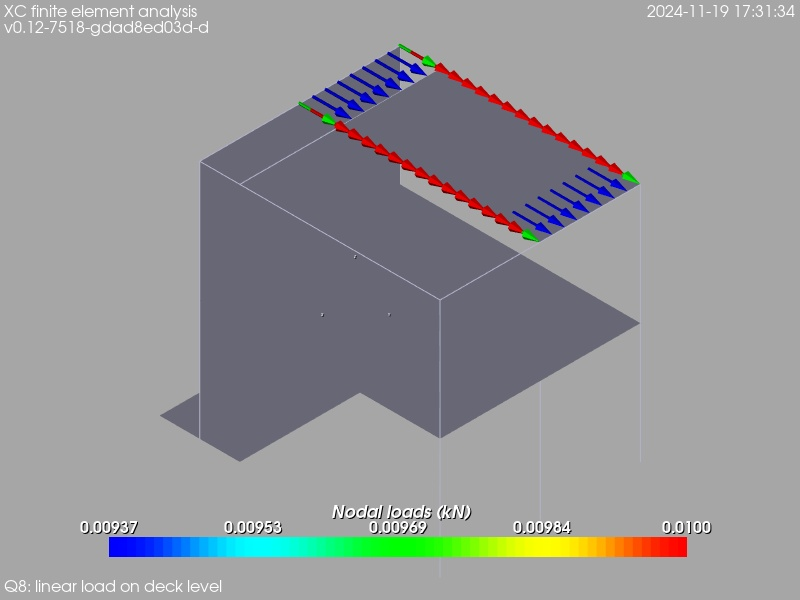
\includegraphics[width=\linewidth]{results/graphics/loads/qlinDeckoverallSet}
\caption{Q8: linear load on deck level , distribución de cargas.}
\label{qlinDeckoverallSet}
\end{center}
\end{figure}
\begin{figure}[ht]
\begin{center}
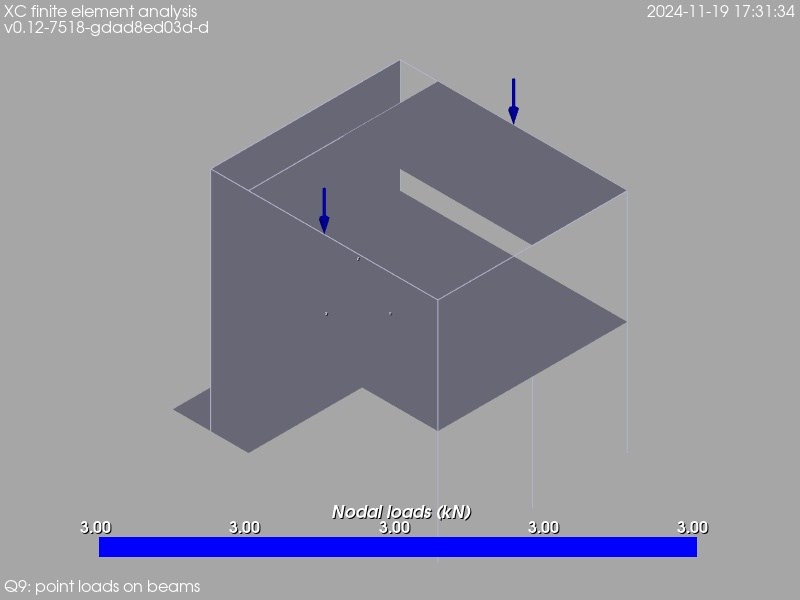
\includegraphics[width=\linewidth]{results/graphics/loads/QpntBeamsoverallSet}
\caption{Q9: point loads on beams, distribución de cargas.}
\label{QpntBeamsoverallSet}
\end{center}
\end{figure}
\begin{figure}[ht]
\begin{center}
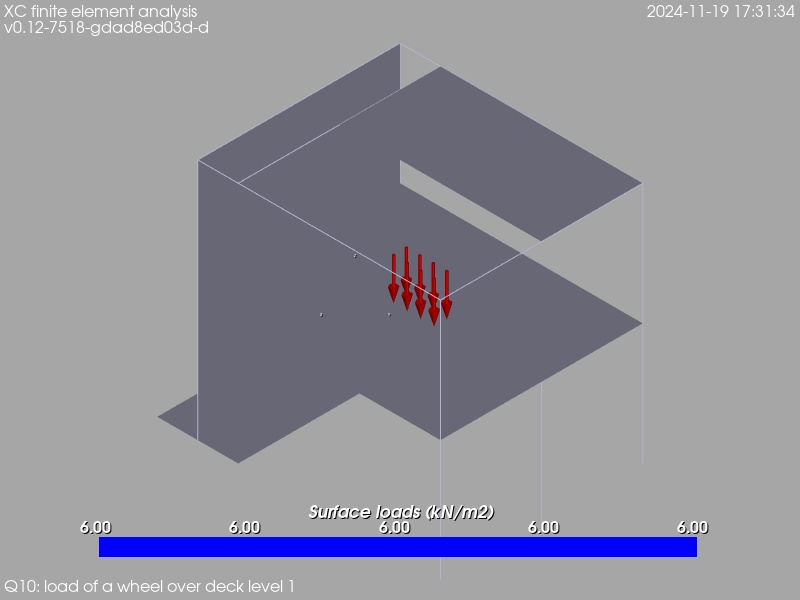
\includegraphics[width=\linewidth]{results/graphics/loads/QwheelDeck1overallSet}
\caption{Q10: load of a wheel over deck level 1, distribución de cargas.}
\label{QwheelDeck1overallSet}
\end{center}
\end{figure}
\begin{figure}[ht]
\begin{center}
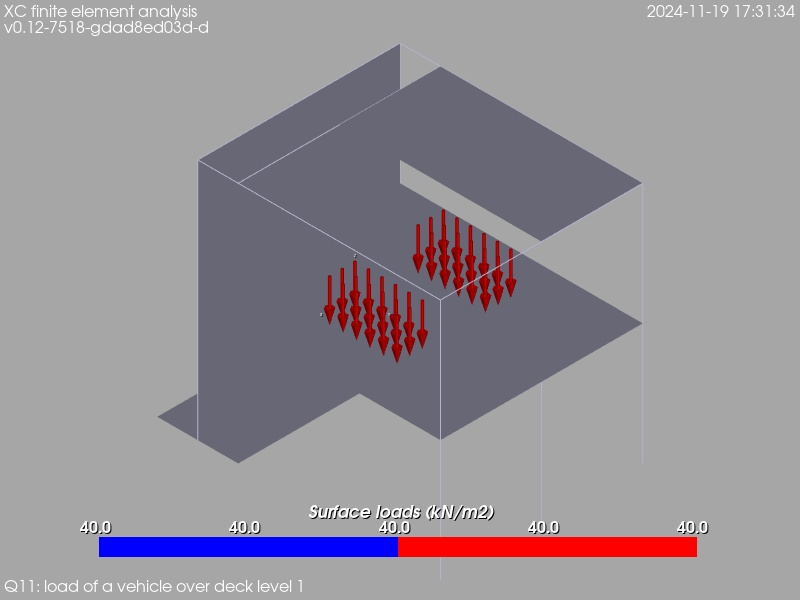
\includegraphics[width=\linewidth]{results/graphics/loads/QvehicleDeck1overallSet}
\caption{Q11: load of a vehicle over deck level 1, distribución de cargas.}
\label{QvehicleDeck1overallSet}
\end{center}
\end{figure}
\begin{figure}[ht]
\begin{center}
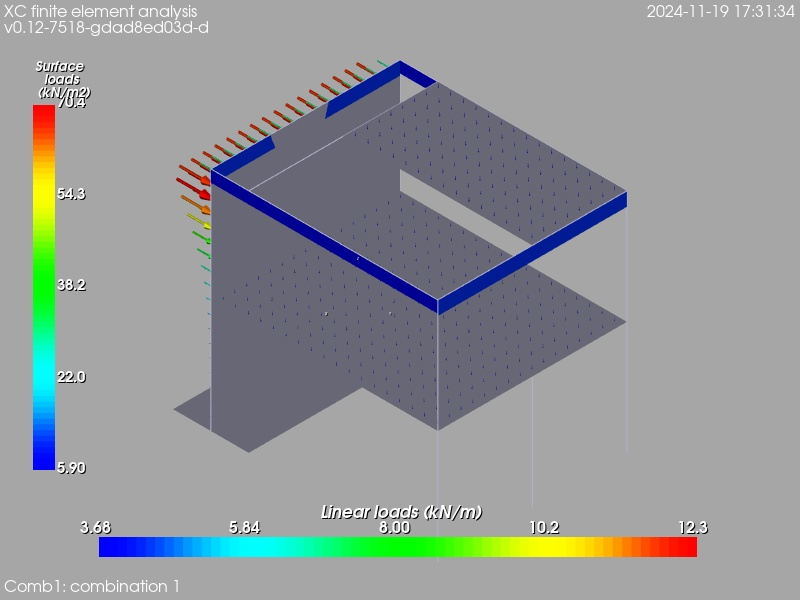
\includegraphics[width=\linewidth]{results/graphics/loads/LS1overallSet}
\caption{Comb1: combination 1, distribución de cargas.}
\label{LS1overallSet}
\end{center}
\end{figure}
\begin{figure}[ht]
\begin{center}
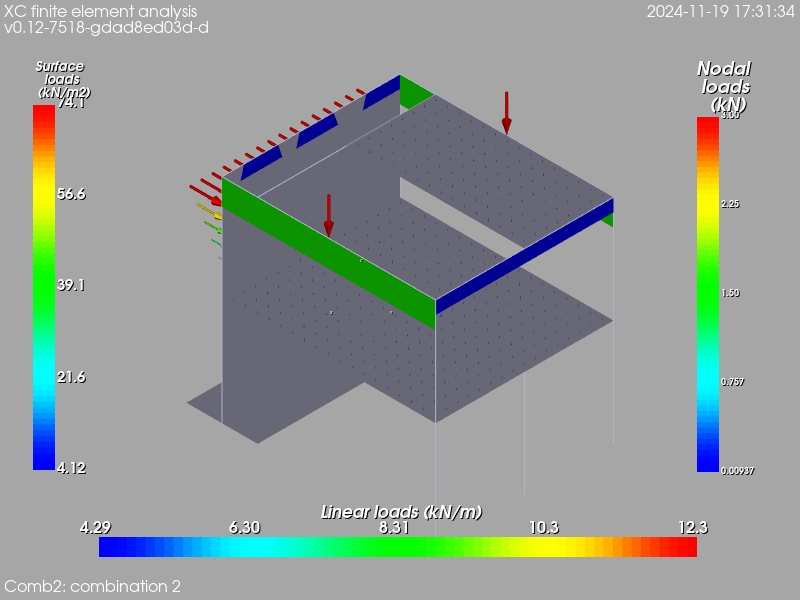
\includegraphics[width=\linewidth]{results/graphics/loads/LS2overallSet}
\caption{Comb2: combination 2, distribución de cargas.}
\label{LS2overallSet}
\end{center}
\end{figure}

\clearpage
\section{Desplazamientos en hipótesis simples de carga}
\begin{figure}[ht]
\begin{center}
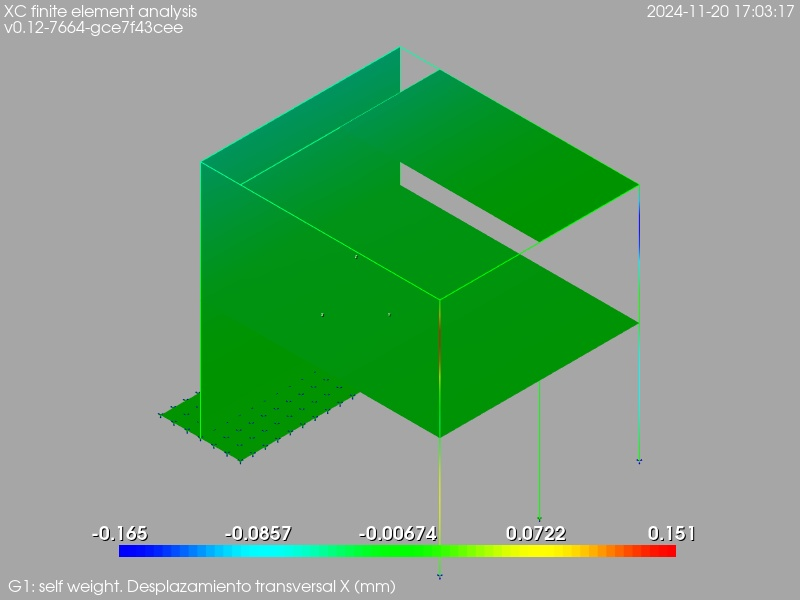
\includegraphics[width=\linewidth]{results/graphics/resSimplLC/GselfWeightuX.png}
\caption{ G1: self weight. Desplazamiento transversal X (mm)}
\label{GselfWeightuX}
\end{center}
\end{figure}
\begin{figure}[ht]
\begin{center}
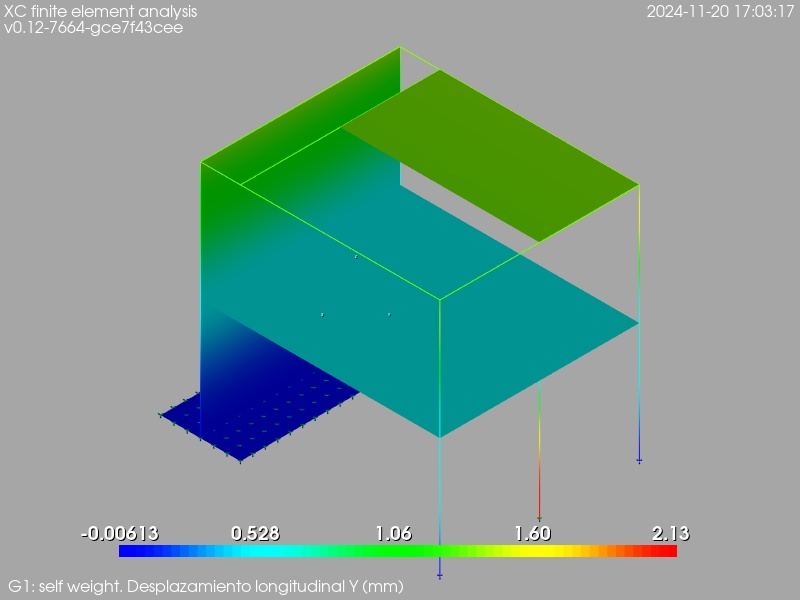
\includegraphics[width=\linewidth]{results/graphics/resSimplLC/GselfWeightuY.png}
\caption{ G1: self weight. Desplazamiento longitudinal Y (mm)}
\label{GselfWeightuY}
\end{center}
\end{figure}
\begin{figure}[ht]
\begin{center}
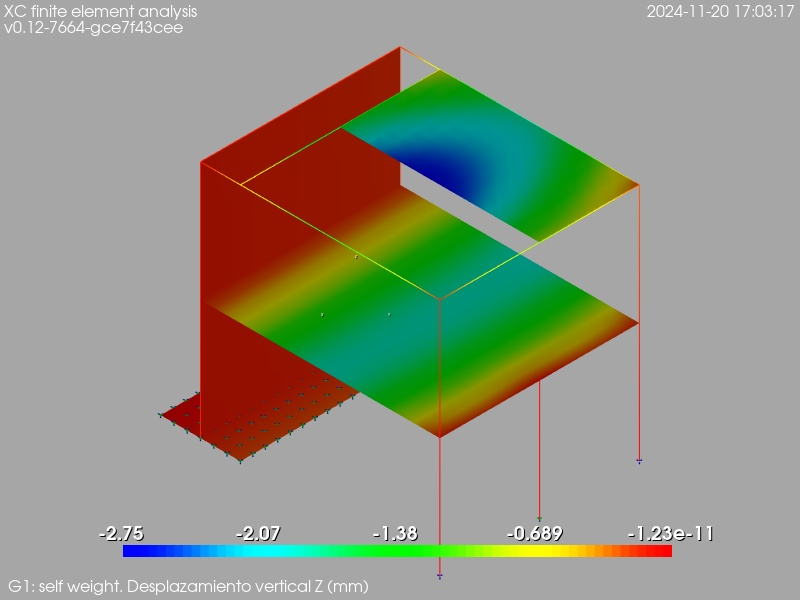
\includegraphics[width=\linewidth]{results/graphics/resSimplLC/GselfWeightuZ.png}
\caption{ G1: self weight. Desplazamiento vertical Z (mm)}
\label{GselfWeightuZ}
\end{center}
\end{figure}
\begin{figure}[ht]
\begin{center}
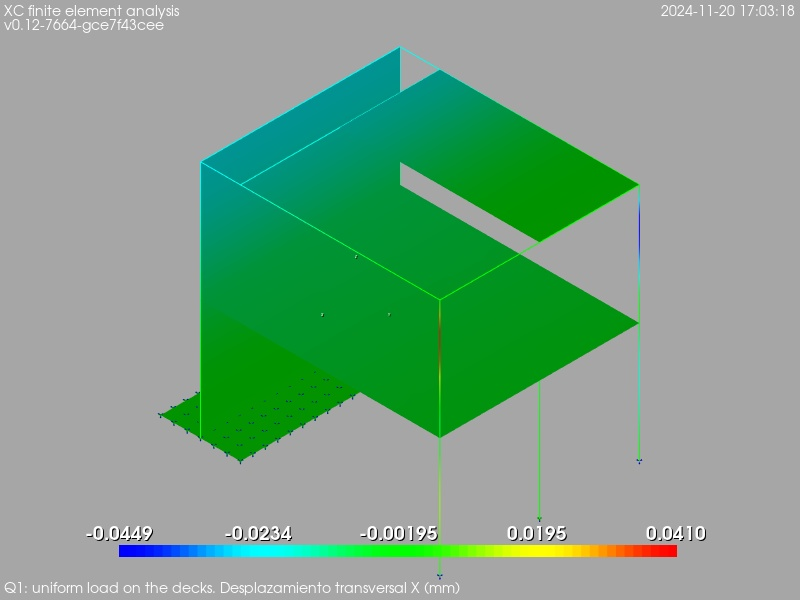
\includegraphics[width=\linewidth]{results/graphics/resSimplLC/QdecksuX.png}
\caption{Q1: uniform load on the decks. Desplazamiento transversal X (mm)}
\label{QdecksuX}
\end{center}
\end{figure}
\begin{figure}[ht]
\begin{center}
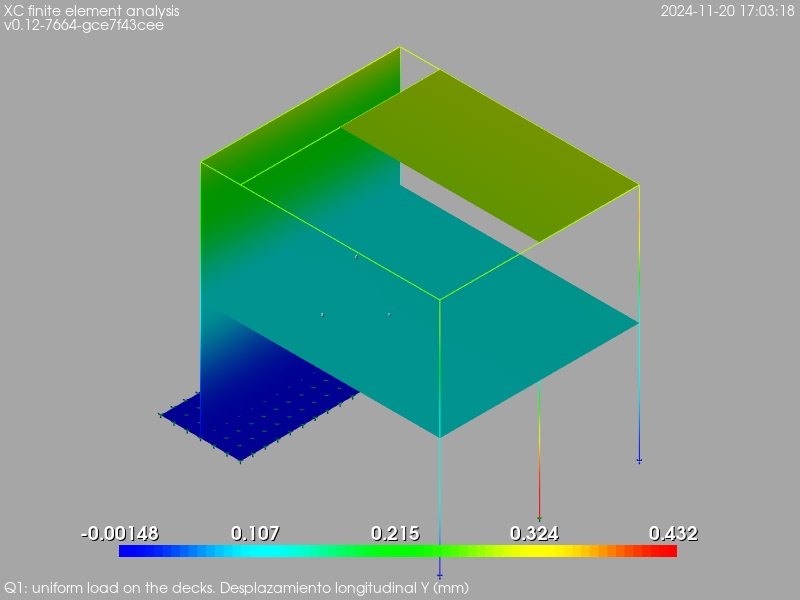
\includegraphics[width=\linewidth]{results/graphics/resSimplLC/QdecksuY.png}
\caption{Q1: uniform load on the decks. Desplazamiento longitudinal Y (mm)}
\label{QdecksuY}
\end{center}
\end{figure}
\begin{figure}[ht]
\begin{center}
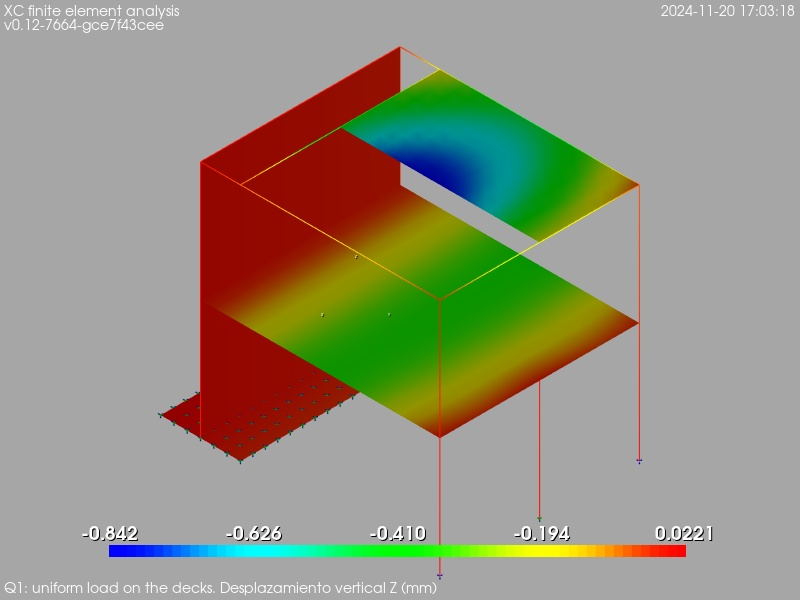
\includegraphics[width=\linewidth]{results/graphics/resSimplLC/QdecksuZ.png}
\caption{Q1: uniform load on the decks. Desplazamiento vertical Z (mm)}
\label{QdecksuZ}
\end{center}
\end{figure}
\begin{figure}[ht]
\begin{center}
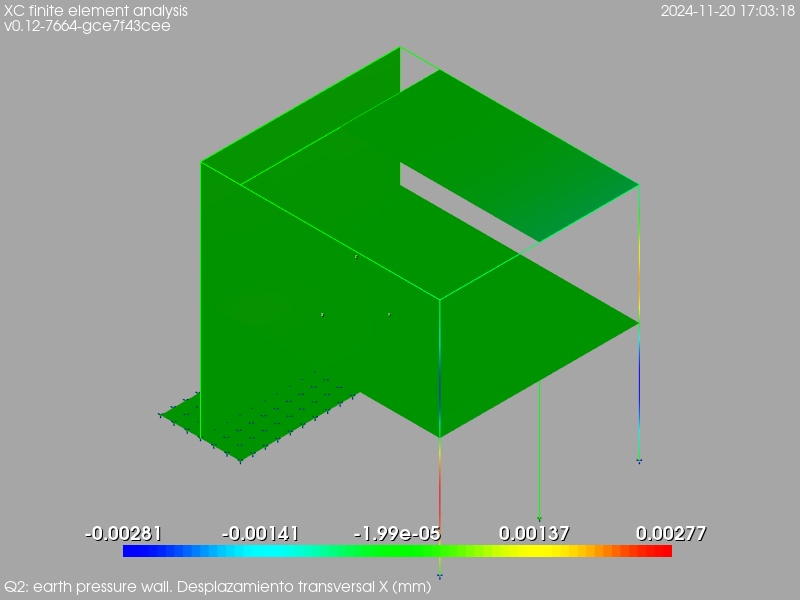
\includegraphics[width=\linewidth]{results/graphics/resSimplLC/QearthPressWalluX.png}
\caption{Q2: earth pressure wall. Desplazamiento transversal X (mm)}
\label{QearthPressWalluX}
\end{center}
\end{figure}
\begin{figure}[ht]
\begin{center}
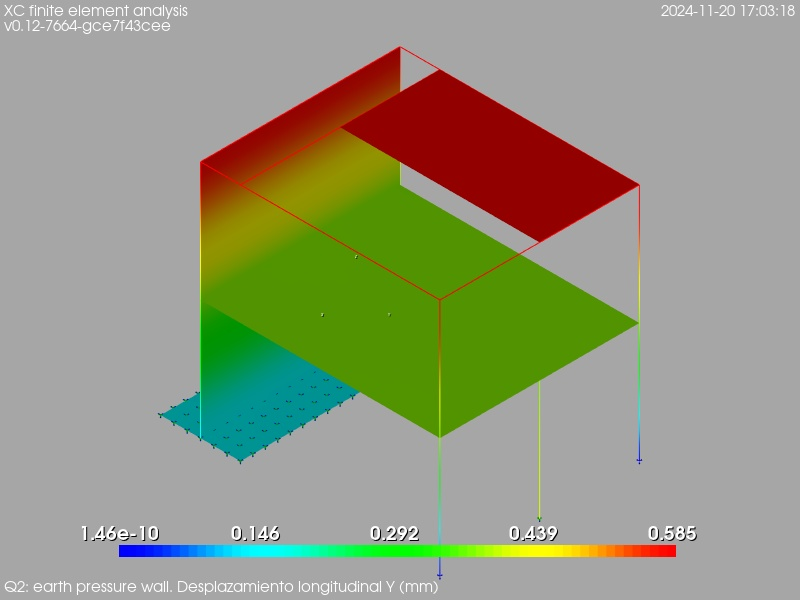
\includegraphics[width=\linewidth]{results/graphics/resSimplLC/QearthPressWalluY.png}
\caption{Q2: earth pressure wall. Desplazamiento longitudinal Y (mm)}
\label{QearthPressWalluY}
\end{center}
\end{figure}
\begin{figure}[ht]
\begin{center}
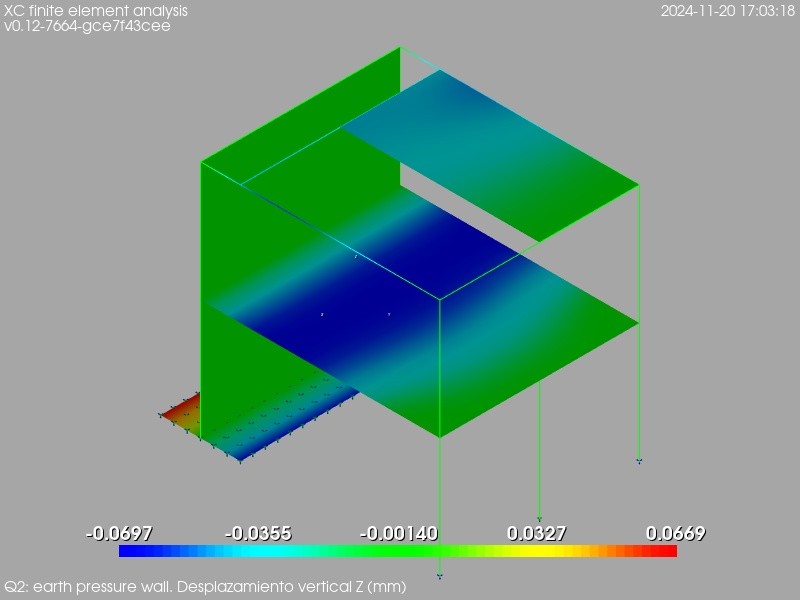
\includegraphics[width=\linewidth]{results/graphics/resSimplLC/QearthPressWalluZ.png}
\caption{Q2: earth pressure wall. Desplazamiento vertical Z (mm)}
\label{QearthPressWalluZ}
\end{center}
\end{figure}
\begin{figure}[ht]
\begin{center}
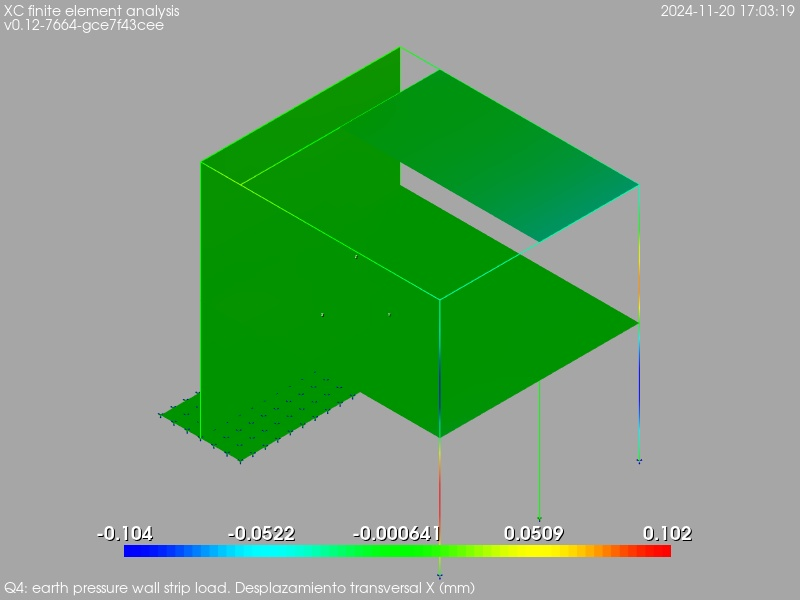
\includegraphics[width=\linewidth]{results/graphics/resSimplLC/QearthPWallStrLuX.png}
\caption{Q4: earth pressure wall strip load. Desplazamiento transversal X (mm)}
\label{QearthPWallStrLuX}
\end{center}
\end{figure}
\begin{figure}[ht]
\begin{center}
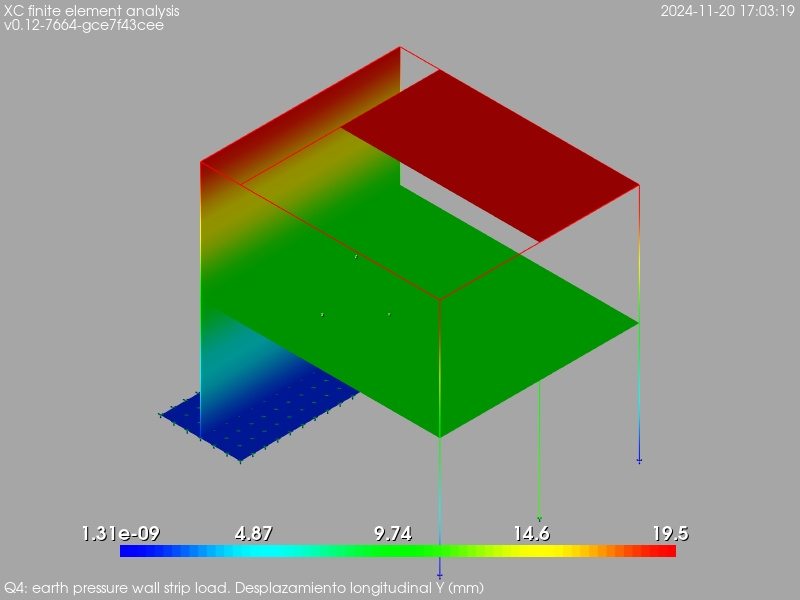
\includegraphics[width=\linewidth]{results/graphics/resSimplLC/QearthPWallStrLuY.png}
\caption{Q4: earth pressure wall strip load. Desplazamiento longitudinal Y (mm)}
\label{QearthPWallStrLuY}
\end{center}
\end{figure}
\begin{figure}[ht]
\begin{center}
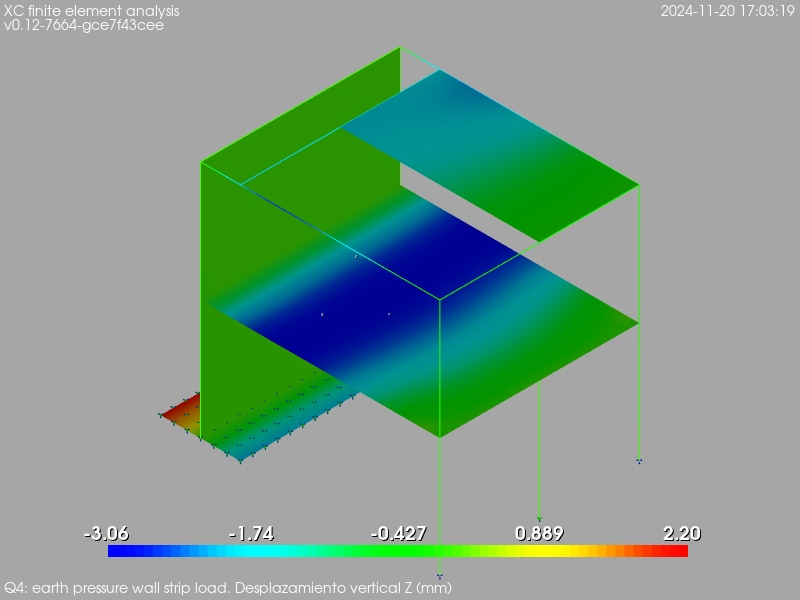
\includegraphics[width=\linewidth]{results/graphics/resSimplLC/QearthPWallStrLuZ.png}
\caption{Q4: earth pressure wall strip load. Desplazamiento vertical Z (mm)}
\label{QearthPWallStrLuZ}
\end{center}
\end{figure}
\begin{figure}[ht]
\begin{center}
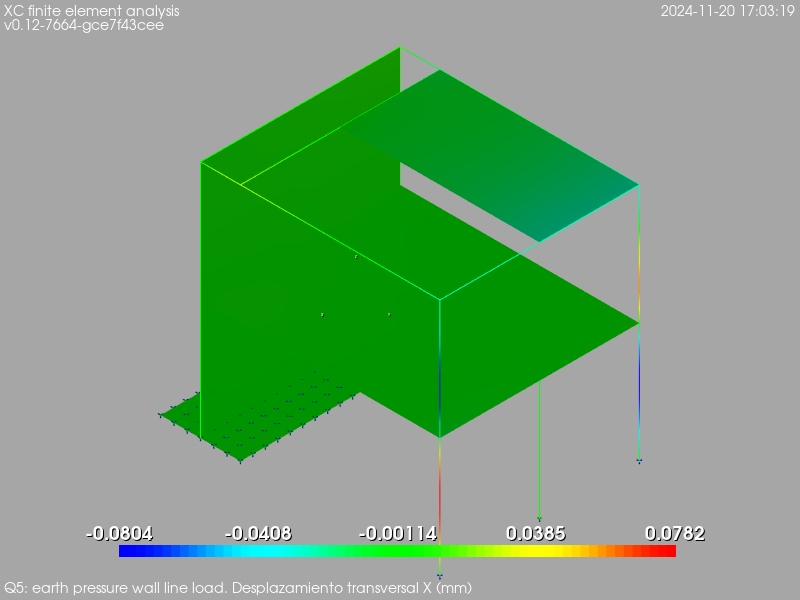
\includegraphics[width=\linewidth]{results/graphics/resSimplLC/QearthPWallLinLuX.png}
\caption{Q5: earth pressure wall line load. Desplazamiento transversal X (mm)}
\label{QearthPWallLinLuX}
\end{center}
\end{figure}
\begin{figure}[ht]
\begin{center}
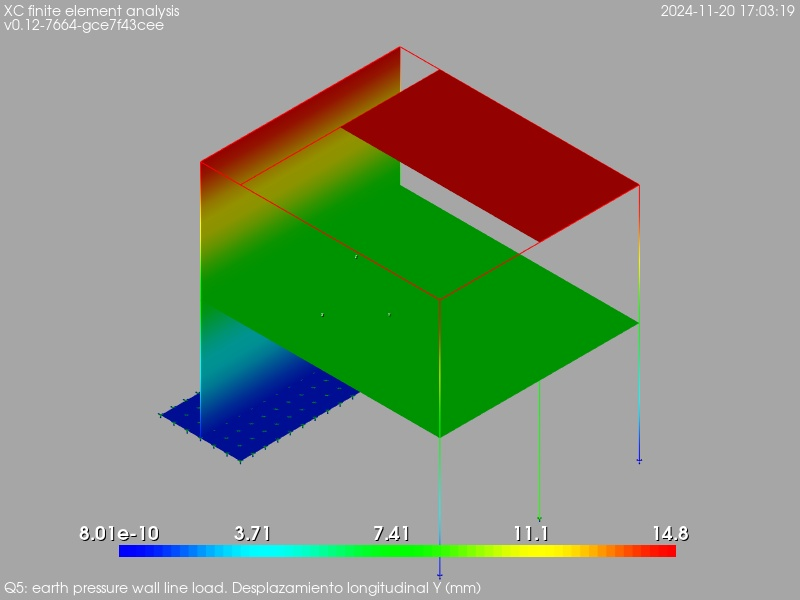
\includegraphics[width=\linewidth]{results/graphics/resSimplLC/QearthPWallLinLuY.png}
\caption{Q5: earth pressure wall line load. Desplazamiento longitudinal Y (mm)}
\label{QearthPWallLinLuY}
\end{center}
\end{figure}
\begin{figure}[ht]
\begin{center}
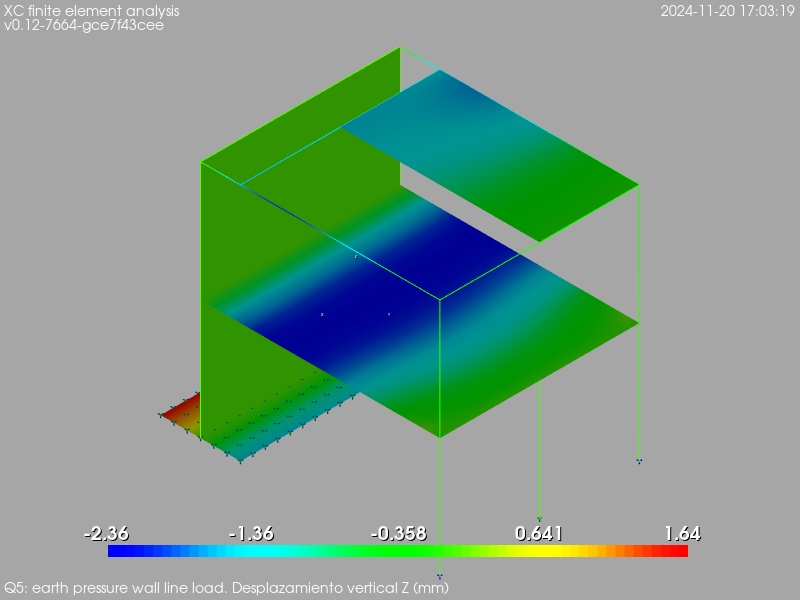
\includegraphics[width=\linewidth]{results/graphics/resSimplLC/QearthPWallLinLuZ.png}
\caption{Q5: earth pressure wall line load. Desplazamiento vertical Z (mm)}
\label{QearthPWallLinLuZ}
\end{center}
\end{figure}
\begin{figure}[ht]
\begin{center}
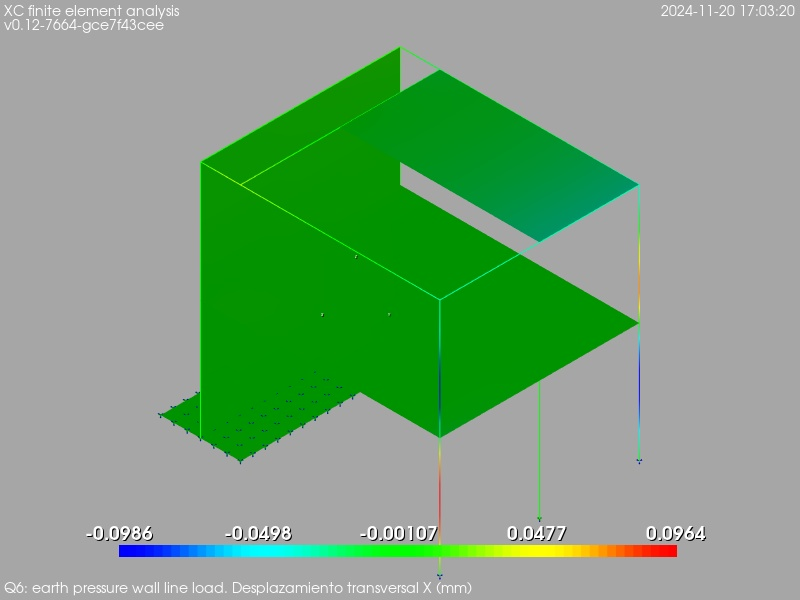
\includegraphics[width=\linewidth]{results/graphics/resSimplLC/QearthPWallHrzLuX.png}
\caption{Q6: earth pressure wall line load. Desplazamiento transversal X (mm)}
\label{QearthPWallHrzLuX}
\end{center}
\end{figure}
\begin{figure}[ht]
\begin{center}
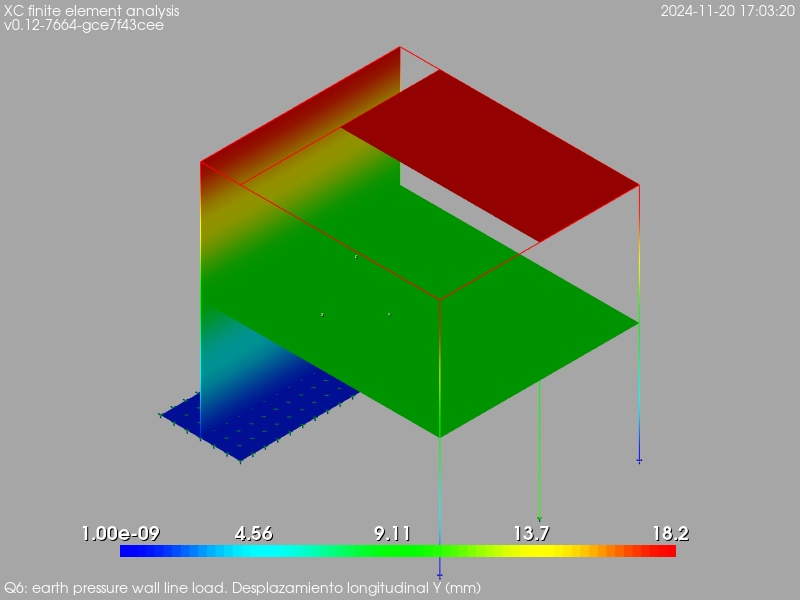
\includegraphics[width=\linewidth]{results/graphics/resSimplLC/QearthPWallHrzLuY.png}
\caption{Q6: earth pressure wall line load. Desplazamiento longitudinal Y (mm)}
\label{QearthPWallHrzLuY}
\end{center}
\end{figure}
\begin{figure}[ht]
\begin{center}
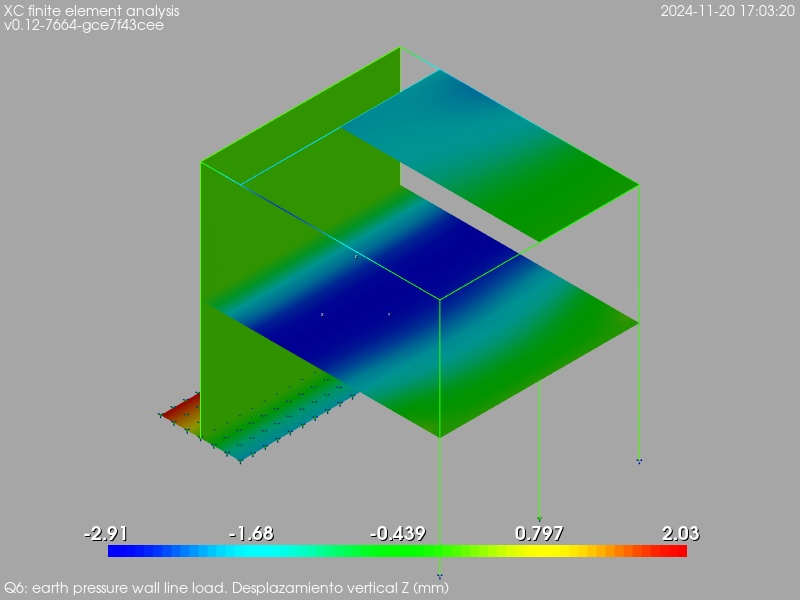
\includegraphics[width=\linewidth]{results/graphics/resSimplLC/QearthPWallHrzLuZ.png}
\caption{Q6: earth pressure wall line load. Desplazamiento vertical Z (mm)}
\label{QearthPWallHrzLuZ}
\end{center}
\end{figure}
\begin{figure}[ht]
\begin{center}
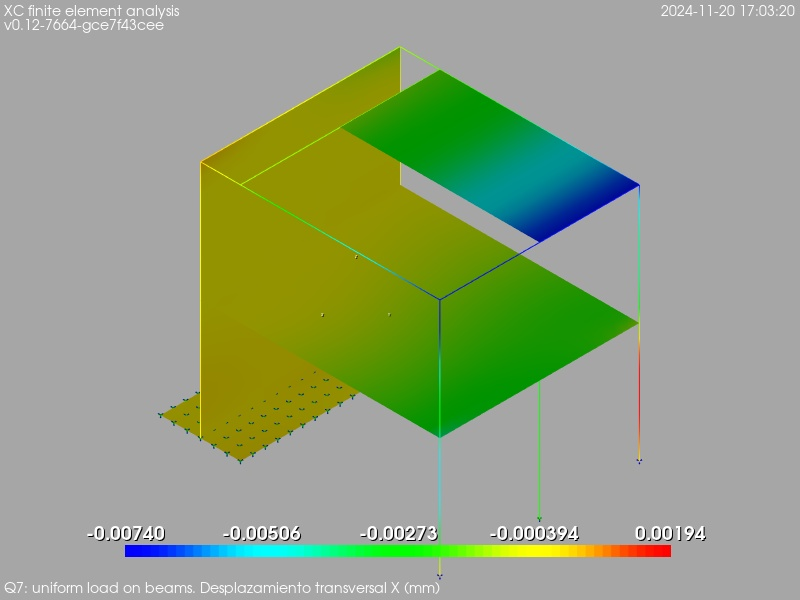
\includegraphics[width=\linewidth]{results/graphics/resSimplLC/qunifBeamsuX.png}
\caption{Q7: uniform load on beams. Desplazamiento transversal X (mm)}
\label{qunifBeamsuX}
\end{center}
\end{figure}
\begin{figure}[ht]
\begin{center}
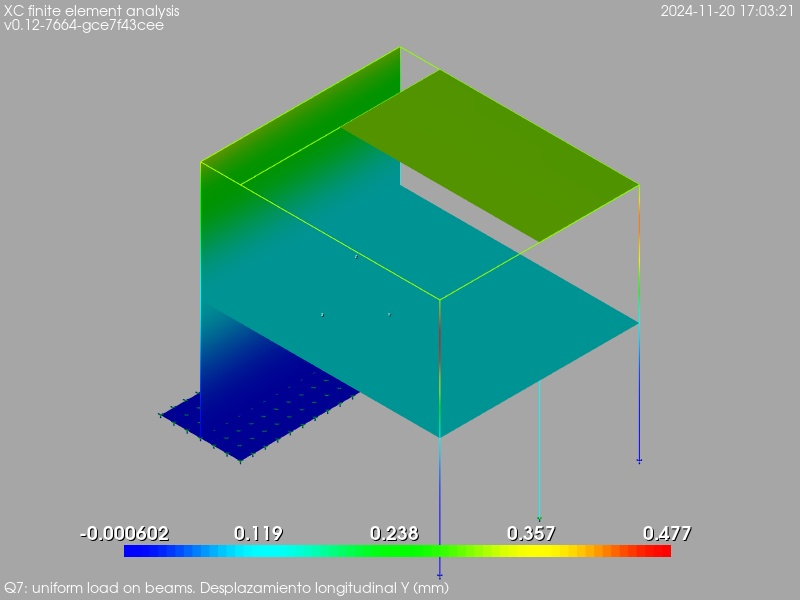
\includegraphics[width=\linewidth]{results/graphics/resSimplLC/qunifBeamsuY.png}
\caption{Q7: uniform load on beams. Desplazamiento longitudinal Y (mm)}
\label{qunifBeamsuY}
\end{center}
\end{figure}
\begin{figure}[ht]
\begin{center}
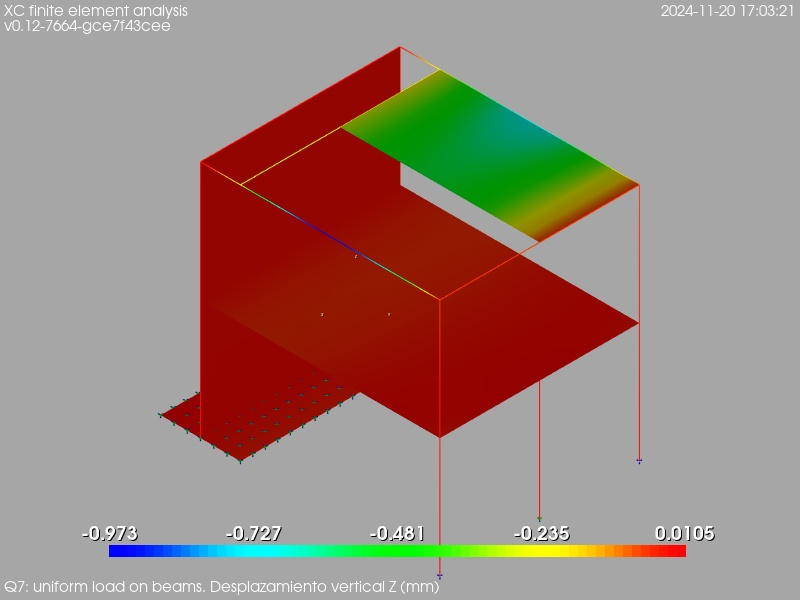
\includegraphics[width=\linewidth]{results/graphics/resSimplLC/qunifBeamsuZ.png}
\caption{Q7: uniform load on beams. Desplazamiento vertical Z (mm)}
\label{qunifBeamsuZ}
\end{center}
\end{figure}
\begin{figure}[ht]
\begin{center}
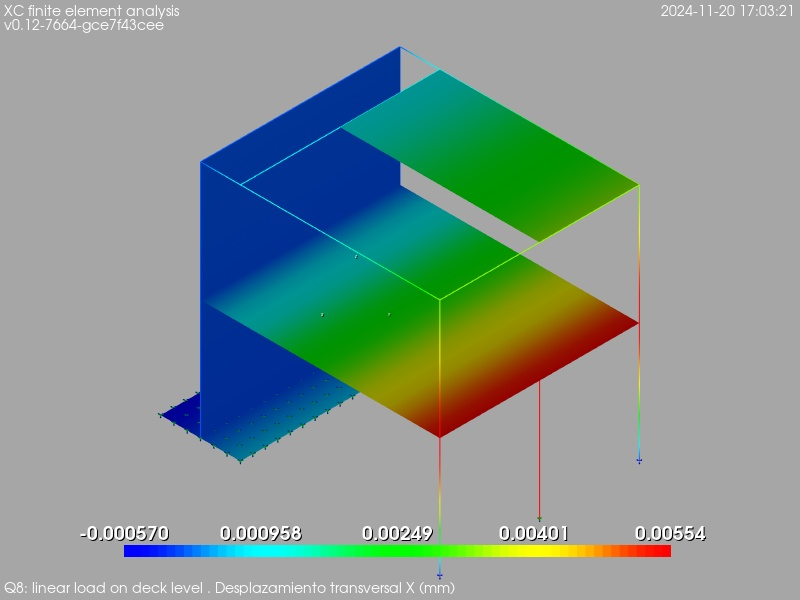
\includegraphics[width=\linewidth]{results/graphics/resSimplLC/qlinDeckuX.png}
\caption{Q8: linear load on deck level . Desplazamiento transversal X (mm)}
\label{qlinDeckuX}
\end{center}
\end{figure}
\begin{figure}[ht]
\begin{center}
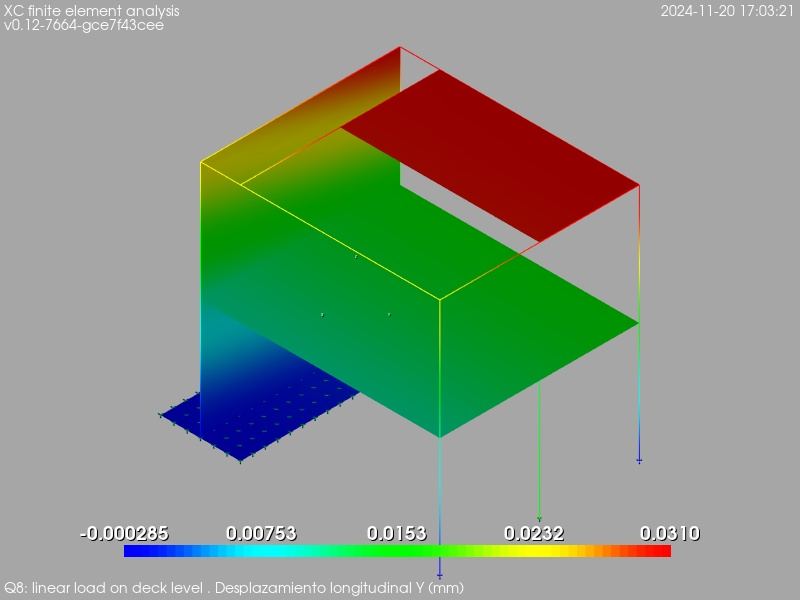
\includegraphics[width=\linewidth]{results/graphics/resSimplLC/qlinDeckuY.png}
\caption{Q8: linear load on deck level . Desplazamiento longitudinal Y (mm)}
\label{qlinDeckuY}
\end{center}
\end{figure}
\begin{figure}[ht]
\begin{center}
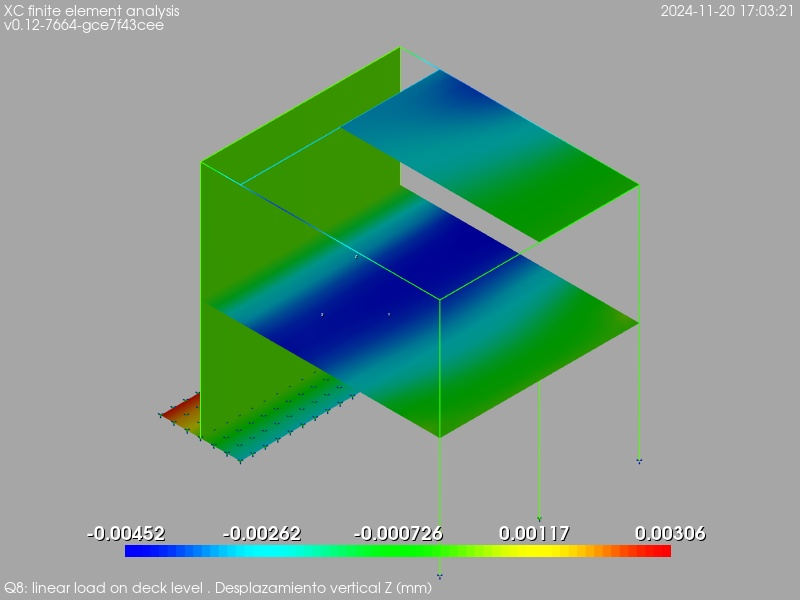
\includegraphics[width=\linewidth]{results/graphics/resSimplLC/qlinDeckuZ.png}
\caption{Q8: linear load on deck level . Desplazamiento vertical Z (mm)}
\label{qlinDeckuZ}
\end{center}
\end{figure}
\begin{figure}[ht]
\begin{center}
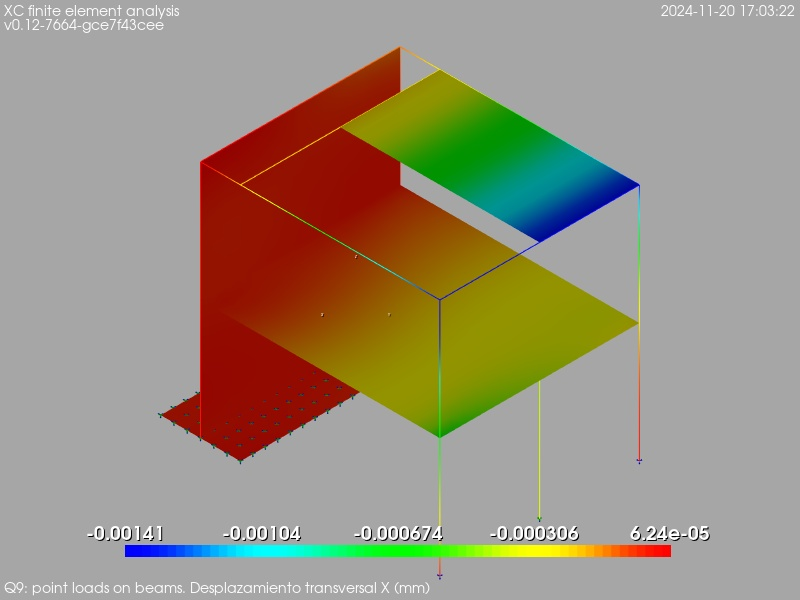
\includegraphics[width=\linewidth]{results/graphics/resSimplLC/QpntBeamsuX.png}
\caption{Q9: point loads on beams. Desplazamiento transversal X (mm)}
\label{QpntBeamsuX}
\end{center}
\end{figure}
\begin{figure}[ht]
\begin{center}
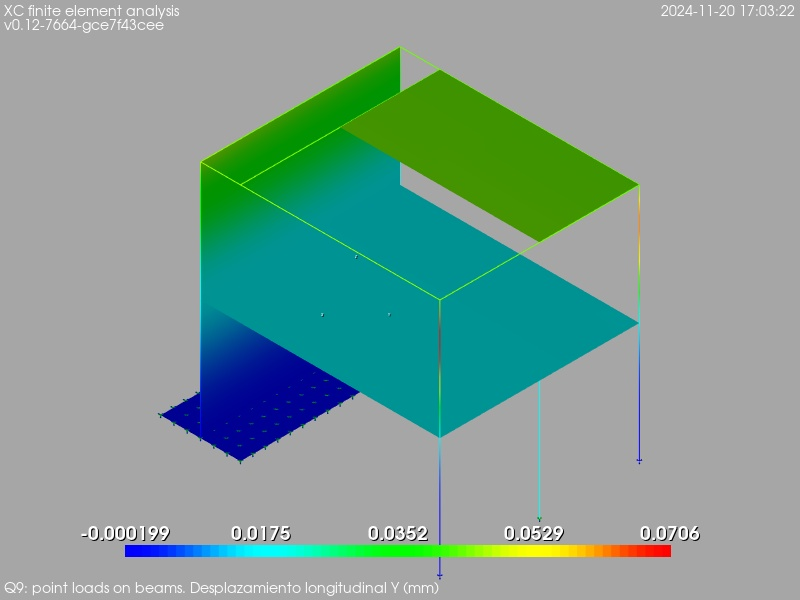
\includegraphics[width=\linewidth]{results/graphics/resSimplLC/QpntBeamsuY.png}
\caption{Q9: point loads on beams. Desplazamiento longitudinal Y (mm)}
\label{QpntBeamsuY}
\end{center}
\end{figure}
\begin{figure}[ht]
\begin{center}
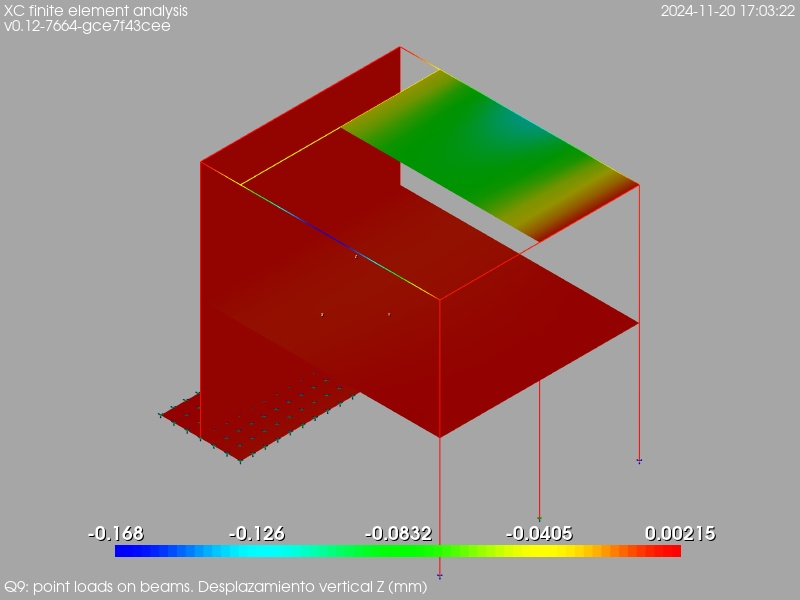
\includegraphics[width=\linewidth]{results/graphics/resSimplLC/QpntBeamsuZ.png}
\caption{Q9: point loads on beams. Desplazamiento vertical Z (mm)}
\label{QpntBeamsuZ}
\end{center}
\end{figure}
\begin{figure}[ht]
\begin{center}
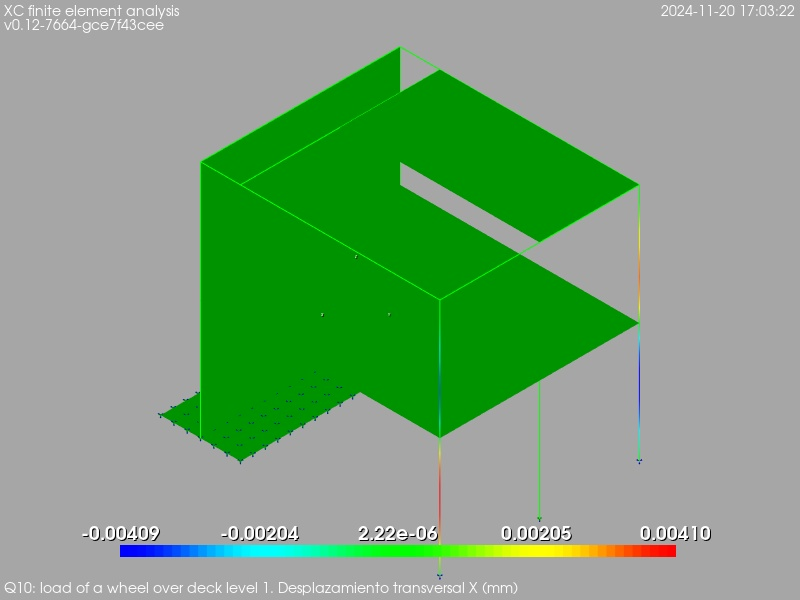
\includegraphics[width=\linewidth]{results/graphics/resSimplLC/QwheelDeck1uX.png}
\caption{Q10: load of a wheel over deck level 1. Desplazamiento transversal X (mm)}
\label{QwheelDeck1uX}
\end{center}
\end{figure}
\begin{figure}[ht]
\begin{center}
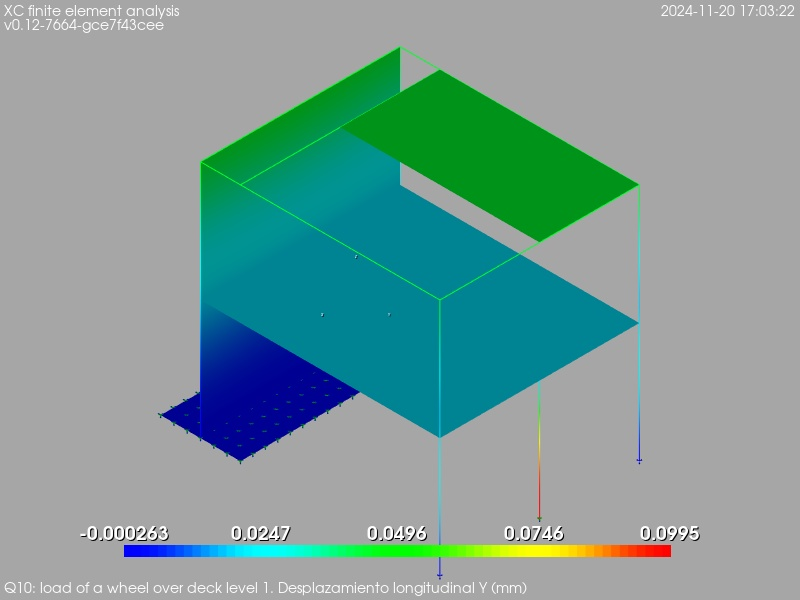
\includegraphics[width=\linewidth]{results/graphics/resSimplLC/QwheelDeck1uY.png}
\caption{Q10: load of a wheel over deck level 1. Desplazamiento longitudinal Y (mm)}
\label{QwheelDeck1uY}
\end{center}
\end{figure}
\begin{figure}[ht]
\begin{center}
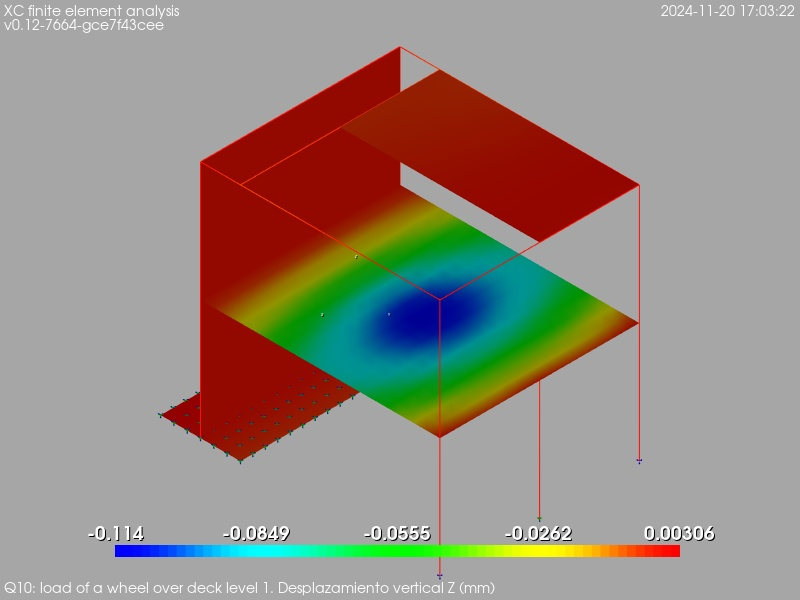
\includegraphics[width=\linewidth]{results/graphics/resSimplLC/QwheelDeck1uZ.png}
\caption{Q10: load of a wheel over deck level 1. Desplazamiento vertical Z (mm)}
\label{QwheelDeck1uZ}
\end{center}
\end{figure}
\begin{figure}[ht]
\begin{center}
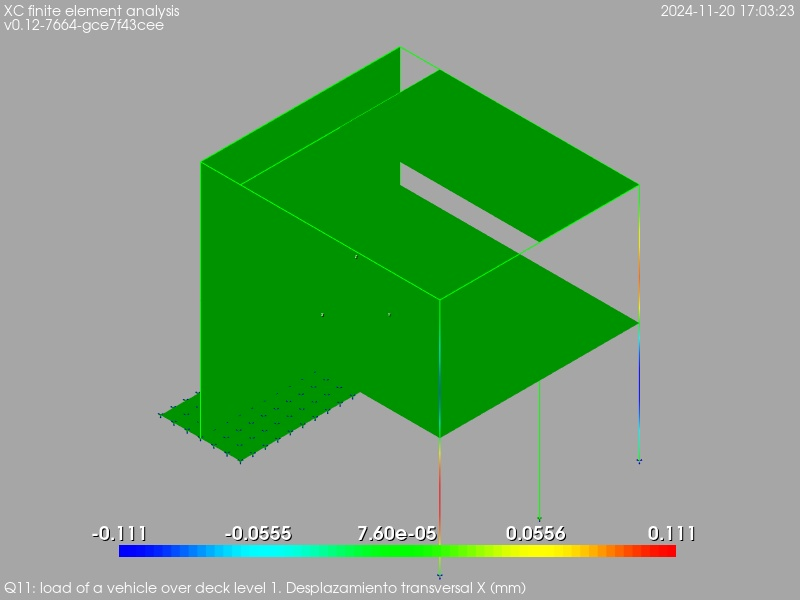
\includegraphics[width=\linewidth]{results/graphics/resSimplLC/QvehicleDeck1uX.png}
\caption{Q11: load of a vehicle over deck level 1. Desplazamiento transversal X (mm)}
\label{QvehicleDeck1uX}
\end{center}
\end{figure}
\begin{figure}[ht]
\begin{center}
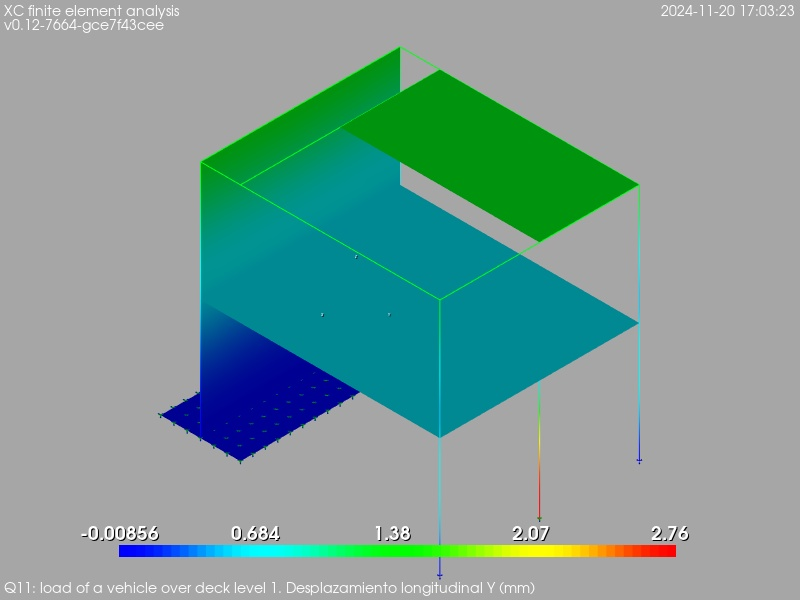
\includegraphics[width=\linewidth]{results/graphics/resSimplLC/QvehicleDeck1uY.png}
\caption{Q11: load of a vehicle over deck level 1. Desplazamiento longitudinal Y (mm)}
\label{QvehicleDeck1uY}
\end{center}
\end{figure}
\begin{figure}[ht]
\begin{center}
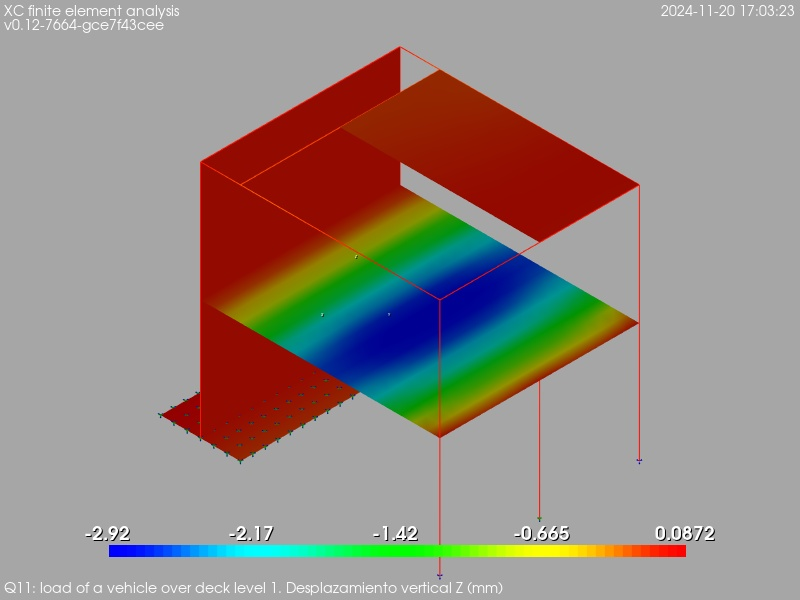
\includegraphics[width=\linewidth]{results/graphics/resSimplLC/QvehicleDeck1uZ.png}
\caption{Q11: load of a vehicle over deck level 1. Desplazamiento vertical Z (mm)}
\label{QvehicleDeck1uZ}
\end{center}
\end{figure}
\begin{figure}[ht]
\begin{center}
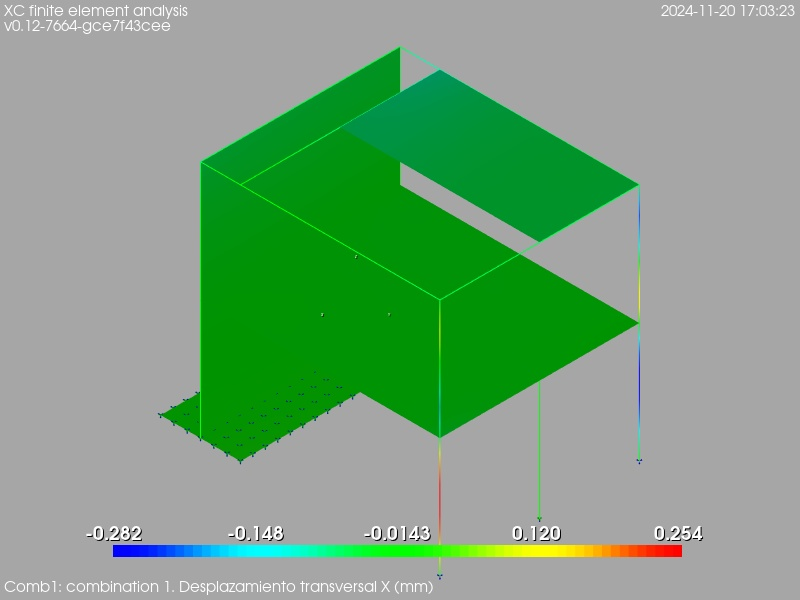
\includegraphics[width=\linewidth]{results/graphics/resSimplLC/LS1uX.png}
\caption{Comb1: combination 1. Desplazamiento transversal X (mm)}
\label{LS1uX}
\end{center}
\end{figure}
\begin{figure}[ht]
\begin{center}
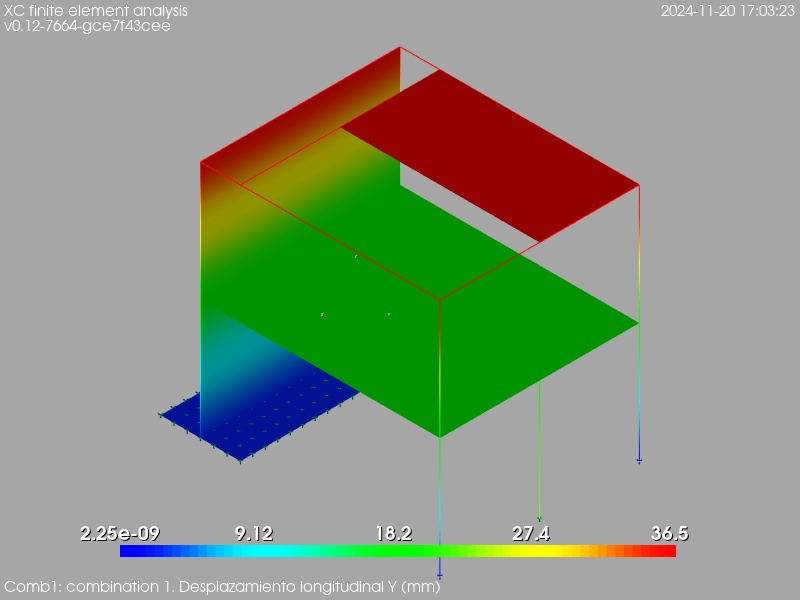
\includegraphics[width=\linewidth]{results/graphics/resSimplLC/LS1uY.png}
\caption{Comb1: combination 1. Desplazamiento longitudinal Y (mm)}
\label{LS1uY}
\end{center}
\end{figure}
\begin{figure}[ht]
\begin{center}
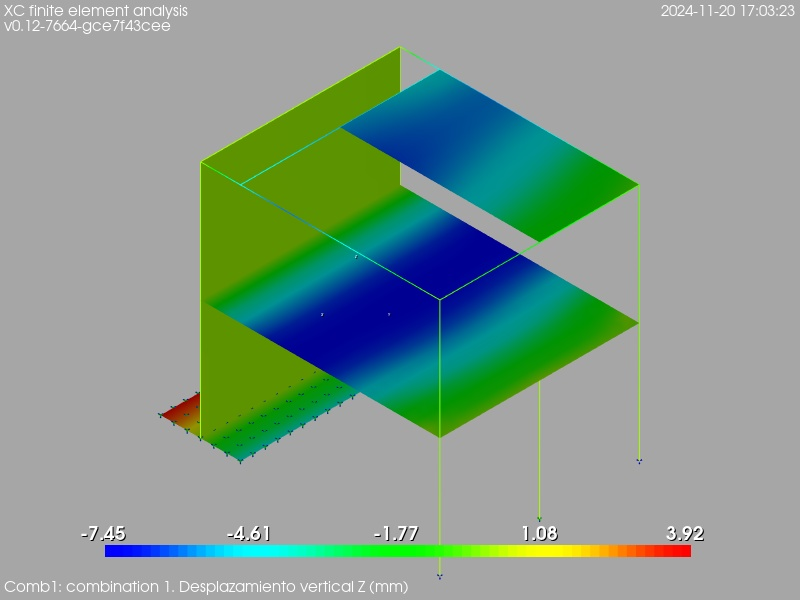
\includegraphics[width=\linewidth]{results/graphics/resSimplLC/LS1uZ.png}
\caption{Comb1: combination 1. Desplazamiento vertical Z (mm)}
\label{LS1uZ}
\end{center}
\end{figure}
\begin{figure}[ht]
\begin{center}
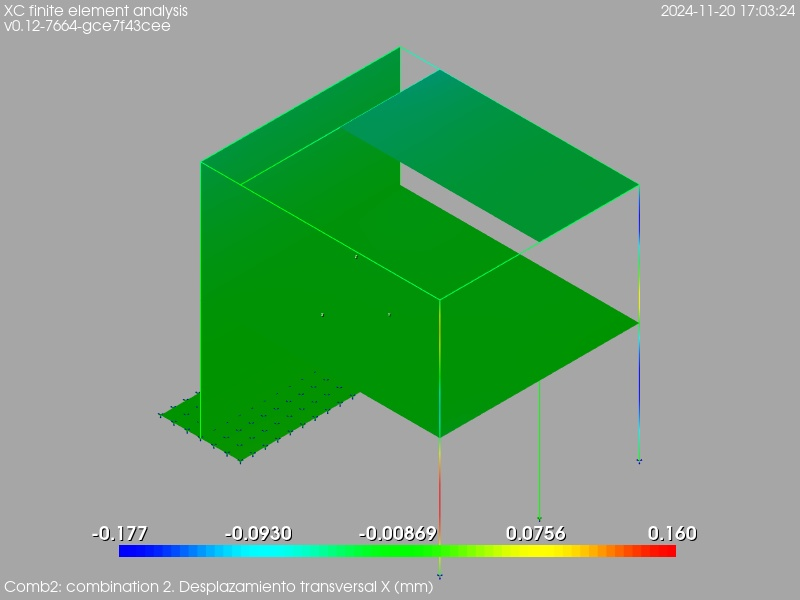
\includegraphics[width=\linewidth]{results/graphics/resSimplLC/LS2uX.png}
\caption{Comb2: combination 2. Desplazamiento transversal X (mm)}
\label{LS2uX}
\end{center}
\end{figure}
\begin{figure}[ht]
\begin{center}
\includegraphics[width=\linewidth]{results/graphics/resSimplLC/LS2uY.png}
\caption{Comb2: combination 2. Desplazamiento longitudinal Y (mm)}
\label{LS2uY}
\end{center}
\end{figure}
\begin{figure}[ht]
\begin{center}
\includegraphics[width=\linewidth]{results/graphics/resSimplLC/LS2uZ.png}
\caption{Comb2: combination 2. Desplazamiento vertical Z (mm)}
\label{LS2uZ}
\end{center}
\end{figure}
\clearpage 

\clearpage
\section{Esfuerzos en hipótesis simples de carga}
\begin{figure}[ht]
\begin{center}
\includegraphics[width=\linewidth]{results/graphics/resSimplLC/GselfWeightcolumnZconcrMz.png}
\caption{ G1: self weightConcrete columns. Momento en eje local Z (kNm)}
\label{GselfWeightcolumnZconcrMz}
\end{center}
\end{figure}
\begin{figure}[ht]
\begin{center}
\includegraphics[width=\linewidth]{results/graphics/resSimplLC/GselfWeightcolumnZconcrVy.png}
\caption{ G1: self weightConcrete columns. Esfuerzo cortante en eje local Y (kN)}
\label{GselfWeightcolumnZconcrVy}
\end{center}
\end{figure}
\begin{figure}[ht]
\begin{center}
\includegraphics[width=\linewidth]{results/graphics/resSimplLC/QdeckscolumnZconcrMz.png}
\caption{Q1: uniform load on the decksConcrete columns. Momento en eje local Z (kNm)}
\label{QdeckscolumnZconcrMz}
\end{center}
\end{figure}
\begin{figure}[ht]
\begin{center}
\includegraphics[width=\linewidth]{results/graphics/resSimplLC/QdeckscolumnZconcrVy.png}
\caption{Q1: uniform load on the decksConcrete columns. Esfuerzo cortante en eje local Y (kN)}
\label{QdeckscolumnZconcrVy}
\end{center}
\end{figure}
\begin{figure}[ht]
\begin{center}
\includegraphics[width=\linewidth]{results/graphics/resSimplLC/QearthPressWallcolumnZconcrMz.png}
\caption{Q2: earth pressure wallConcrete columns. Momento en eje local Z (kNm)}
\label{QearthPressWallcolumnZconcrMz}
\end{center}
\end{figure}
\begin{figure}[ht]
\begin{center}
\includegraphics[width=\linewidth]{results/graphics/resSimplLC/QearthPressWallcolumnZconcrVy.png}
\caption{Q2: earth pressure wallConcrete columns. Esfuerzo cortante en eje local Y (kN)}
\label{QearthPressWallcolumnZconcrVy}
\end{center}
\end{figure}
\begin{figure}[ht]
\begin{center}
\includegraphics[width=\linewidth]{results/graphics/resSimplLC/QearthPWallStrLcolumnZconcrMz.png}
\caption{Q4: earth pressure wall strip loadConcrete columns. Momento en eje local Z (kNm)}
\label{QearthPWallStrLcolumnZconcrMz}
\end{center}
\end{figure}
\begin{figure}[ht]
\begin{center}
\includegraphics[width=\linewidth]{results/graphics/resSimplLC/QearthPWallStrLcolumnZconcrVy.png}
\caption{Q4: earth pressure wall strip loadConcrete columns. Esfuerzo cortante en eje local Y (kN)}
\label{QearthPWallStrLcolumnZconcrVy}
\end{center}
\end{figure}
\begin{figure}[ht]
\begin{center}
\includegraphics[width=\linewidth]{results/graphics/resSimplLC/QearthPWallLinLcolumnZconcrMz.png}
\caption{Q5: earth pressure wall line loadConcrete columns. Momento en eje local Z (kNm)}
\label{QearthPWallLinLcolumnZconcrMz}
\end{center}
\end{figure}
\begin{figure}[ht]
\begin{center}
\includegraphics[width=\linewidth]{results/graphics/resSimplLC/QearthPWallLinLcolumnZconcrVy.png}
\caption{Q5: earth pressure wall line loadConcrete columns. Esfuerzo cortante en eje local Y (kN)}
\label{QearthPWallLinLcolumnZconcrVy}
\end{center}
\end{figure}
\begin{figure}[ht]
\begin{center}
\includegraphics[width=\linewidth]{results/graphics/resSimplLC/QearthPWallHrzLcolumnZconcrMz.png}
\caption{Q6: earth pressure wall line loadConcrete columns. Momento en eje local Z (kNm)}
\label{QearthPWallHrzLcolumnZconcrMz}
\end{center}
\end{figure}
\begin{figure}[ht]
\begin{center}
\includegraphics[width=\linewidth]{results/graphics/resSimplLC/QearthPWallHrzLcolumnZconcrVy.png}
\caption{Q6: earth pressure wall line loadConcrete columns. Esfuerzo cortante en eje local Y (kN)}
\label{QearthPWallHrzLcolumnZconcrVy}
\end{center}
\end{figure}
\begin{figure}[ht]
\begin{center}
\includegraphics[width=\linewidth]{results/graphics/resSimplLC/qunifBeamscolumnZconcrMz.png}
\caption{Q7: uniform load on beamsConcrete columns. Momento en eje local Z (kNm)}
\label{qunifBeamscolumnZconcrMz}
\end{center}
\end{figure}
\begin{figure}[ht]
\begin{center}
\includegraphics[width=\linewidth]{results/graphics/resSimplLC/qunifBeamscolumnZconcrVy.png}
\caption{Q7: uniform load on beamsConcrete columns. Esfuerzo cortante en eje local Y (kN)}
\label{qunifBeamscolumnZconcrVy}
\end{center}
\end{figure}
\begin{figure}[ht]
\begin{center}
\includegraphics[width=\linewidth]{results/graphics/resSimplLC/qlinDeckcolumnZconcrMz.png}
\caption{Q8: linear load on deck level Concrete columns. Momento en eje local Z (kNm)}
\label{qlinDeckcolumnZconcrMz}
\end{center}
\end{figure}
\begin{figure}[ht]
\begin{center}
\includegraphics[width=\linewidth]{results/graphics/resSimplLC/qlinDeckcolumnZconcrVy.png}
\caption{Q8: linear load on deck level Concrete columns. Esfuerzo cortante en eje local Y (kN)}
\label{qlinDeckcolumnZconcrVy}
\end{center}
\end{figure}
\begin{figure}[ht]
\begin{center}
\includegraphics[width=\linewidth]{results/graphics/resSimplLC/QpntBeamscolumnZconcrMz.png}
\caption{Q9: point loads on beamsConcrete columns. Momento en eje local Z (kNm)}
\label{QpntBeamscolumnZconcrMz}
\end{center}
\end{figure}
\begin{figure}[ht]
\begin{center}
\includegraphics[width=\linewidth]{results/graphics/resSimplLC/QpntBeamscolumnZconcrVy.png}
\caption{Q9: point loads on beamsConcrete columns. Esfuerzo cortante en eje local Y (kN)}
\label{QpntBeamscolumnZconcrVy}
\end{center}
\end{figure}
\begin{figure}[ht]
\begin{center}
\includegraphics[width=\linewidth]{results/graphics/resSimplLC/QwheelDeck1columnZconcrMz.png}
\caption{Q10: load of a wheel over deck level 1Concrete columns. Momento en eje local Z (kNm)}
\label{QwheelDeck1columnZconcrMz}
\end{center}
\end{figure}
\begin{figure}[ht]
\begin{center}
\includegraphics[width=\linewidth]{results/graphics/resSimplLC/QwheelDeck1columnZconcrVy.png}
\caption{Q10: load of a wheel over deck level 1Concrete columns. Esfuerzo cortante en eje local Y (kN)}
\label{QwheelDeck1columnZconcrVy}
\end{center}
\end{figure}
\begin{figure}[ht]
\begin{center}
\includegraphics[width=\linewidth]{results/graphics/resSimplLC/QvehicleDeck1columnZconcrMz.png}
\caption{Q11: load of a vehicle over deck level 1Concrete columns. Momento en eje local Z (kNm)}
\label{QvehicleDeck1columnZconcrMz}
\end{center}
\end{figure}
\begin{figure}[ht]
\begin{center}
\includegraphics[width=\linewidth]{results/graphics/resSimplLC/QvehicleDeck1columnZconcrVy.png}
\caption{Q11: load of a vehicle over deck level 1Concrete columns. Esfuerzo cortante en eje local Y (kN)}
\label{QvehicleDeck1columnZconcrVy}
\end{center}
\end{figure}
\begin{figure}[ht]
\begin{center}
\includegraphics[width=\linewidth]{results/graphics/resSimplLC/LS1columnZconcrMz.png}
\caption{Comb1: combination 1Concrete columns. Momento en eje local Z (kNm)}
\label{LS1columnZconcrMz}
\end{center}
\end{figure}
\begin{figure}[ht]
\begin{center}
\includegraphics[width=\linewidth]{results/graphics/resSimplLC/LS1columnZconcrVy.png}
\caption{Comb1: combination 1Concrete columns. Esfuerzo cortante en eje local Y (kN)}
\label{LS1columnZconcrVy}
\end{center}
\end{figure}
\begin{figure}[ht]
\begin{center}
\includegraphics[width=\linewidth]{results/graphics/resSimplLC/LS2columnZconcrMz.png}
\caption{Comb2: combination 2Concrete columns. Momento en eje local Z (kNm)}
\label{LS2columnZconcrMz}
\end{center}
\end{figure}
\begin{figure}[ht]
\begin{center}
\includegraphics[width=\linewidth]{results/graphics/resSimplLC/LS2columnZconcrVy.png}
\caption{Comb2: combination 2Concrete columns. Esfuerzo cortante en eje local Y (kN)}
\label{LS2columnZconcrVy}
\end{center}
\end{figure}
\clearpage 

\clearpage
\section{Materiales y secciones de cálculo}
\begin{center}
\includegraphics[width=120mm]{results/graphics/sections/B500S_design_stress_strain_diagram}
\end{center}
\begin{center}
\includegraphics[width=120mm]{results/graphics/sections/HA30_design_stress_strain_diagram}
\end{center}
%% ****** Packages needed for LaTeX document: ****** 
%%\usepackage{graphicx} %%\postscript includes
%%\usepackage{multirow} %%\multirow command
%%\usepackage{wasysym} %%\permil command
%%\usepackage{gensymb} %%\degree command
\begin{table}
\begin{center}
\begin{tabular}{|c|}
\hline
\begin{large} columnZconcrSect1 \end{large}\\
\hline
cylindric columns Z 1 integration point.\\
\hline
\begin{tabular}{c|l}
\begin{minipage}{85mm}
\vspace{2mm}
\begin{center}
\includegraphics[width=70mm]{results/graphics/sections//columnZconcrSect1}
\end{center}
\vspace{1pt}
\end{minipage} & 
\begin{tabular}{l}
ext. radius: \\
$r_{ext}= 0.40\ m$\\
int. radius: \\
$r_{int}= 0.00\ m$\\
\end{tabular} \\
\end{tabular} \\
\hline
\textbf{Materials - mechanical properties}:\\
\hline
\begin{tabular}{ll}
Concrete: HA30 & Modulus of elasticity: $E_c= 28.58\ GPa$\\
\hline
Steel: B500S & Modulus of elasticity: $E_s= 200.00\ GPa$\\
\end{tabular} \\
\hline
\textbf{Sections - geometric and mechanical characteristics}:\\
\hline
Gross section:\\
\hline
\begin{tabular}{ll}
$A_{gross}= 0.495\ m^2$ & \multirow{3}{*}{Inertia tensor ($cm^4$): $ \left( \begin{array}{ccc}402.12 & 0.00 & 0.00 \\ 0.00 & 195.14 &  0.00 \\ 0.00 &  0.00 & 195.14 \end{array} \right)$} \\
& \\
C.O.G.: $(0.000,0.000)\ m$  & \\
\end{tabular} \\
\hline
Homogenized section:\\
\hline
\begin{tabular}{ll}
$A_{homog.}= 0.539\ m^2$ & \multirow{3}{*}{Inertia tensor ($cm^4$): $ \left( \begin{array}{ccc}402.12 & 0.00 & 0.00 \\ 0.00 & 220.17 &  0.00 \\ 0.00 &  0.00 & 223.99 \end{array} \right)$} \\
& \\
C.O.G.: $(0.002,0.000)\ m$  & \\
\end{tabular} \\
\hline
\textbf{Passive reinforcement}:\\
\hline
\begin{tabular}{ll}
Total area $A_s=43.98\ cm^2$ & Geometric quantity $\rho= 8.88\permil$\\
\end{tabular} \\
\hline
Layers of main reinforcement:\\
\hline
\begin{tabular}{cccccccc}
Id & N$^o$ bars & $\phi$ & area & c. geom. & eff. cover & $y_{COG}$ & $z_{COG}$\\
 &  & $(mm)$ & $(cm^2)$ & $(\permil)$ & $(cm)$ & $(m)$ & $(m)$\\
\hline
 & 14 & 20 &  3.14 & 0.63 &  4.6 & 0.025 & 0.000\\
\end{tabular} \\
\hline
Layers of shear reinforcement:\\
\hline
\begin{tabular}{cccccccc}
Id & N$^o$ branch & $\phi$ & area & spac. & area/m & $\alpha$ & $\beta$\\
 &  & $(mm)$ & $(cm^2)$ & $(cm)$ & $(cm^2/m)$ & $( \degree)$ & $( \degree)$\\
\hline
 & 2 & 10 & 10.47 & 15.0 & 69.81 & 90.0 & 45.0\\
\end{tabular} \\
\hline
\end{tabular}
\end{center}
\caption{cylindric columns Z 1 integration point. (columnZconcrSect1).} \label{tb_columnZconcrSect1}
\end{table}
\begin{center}
\includegraphics[width=80mm]{results/graphics/sections/columnZconcrSect1NMy}
\end{center}
\begin{center}
\includegraphics[width=80mm]{results/graphics/sections/columnZconcrSect1NMz}
\end{center}
%% ****** Packages needed for LaTeX document: ****** 
%%\usepackage{graphicx} %%\postscript includes
%%\usepackage{multirow} %%\multirow command
%%\usepackage{wasysym} %%\permil command
%%\usepackage{gensymb} %%\degree command
\begin{table}
\begin{center}
\begin{tabular}{|c|}
\hline
\begin{large} columnZconcrSect2 \end{large}\\
\hline
cylindric columns Z 2 integration point.\\
\hline
\begin{tabular}{c|l}
\begin{minipage}{85mm}
\vspace{2mm}
\begin{center}
\includegraphics[width=70mm]{results/graphics/sections//columnZconcrSect2}
\end{center}
\vspace{1pt}
\end{minipage} & 
\begin{tabular}{l}
ext. radius: \\
$r_{ext}= 0.40\ m$\\
int. radius: \\
$r_{int}= 0.00\ m$\\
\end{tabular} \\
\end{tabular} \\
\hline
\textbf{Materials - mechanical properties}:\\
\hline
\begin{tabular}{ll}
Concrete: HA30 & Modulus of elasticity: $E_c= 28.58\ GPa$\\
\hline
Steel: B500S & Modulus of elasticity: $E_s= 200.00\ GPa$\\
\end{tabular} \\
\hline
\textbf{Sections - geometric and mechanical characteristics}:\\
\hline
Gross section:\\
\hline
\begin{tabular}{ll}
$A_{gross}= 0.495\ m^2$ & \multirow{3}{*}{Inertia tensor ($cm^4$): $ \left( \begin{array}{ccc}402.12 & 0.00 & 0.00 \\ 0.00 & 195.14 &  0.00 \\ 0.00 &  0.00 & 195.14 \end{array} \right)$} \\
& \\
C.O.G.: $(0.000,0.000)\ m$  & \\
\end{tabular} \\
\hline
Homogenized section:\\
\hline
\begin{tabular}{ll}
$A_{homog.}= 0.539\ m^2$ & \multirow{3}{*}{Inertia tensor ($cm^4$): $ \left( \begin{array}{ccc}402.12 & 0.00 & 0.00 \\ 0.00 & 220.17 &  0.00 \\ 0.00 &  0.00 & 223.99 \end{array} \right)$} \\
& \\
C.O.G.: $(0.002,0.000)\ m$  & \\
\end{tabular} \\
\hline
\textbf{Passive reinforcement}:\\
\hline
\begin{tabular}{ll}
Total area $A_s=43.98\ cm^2$ & Geometric quantity $\rho= 8.88\permil$\\
\end{tabular} \\
\hline
Layers of main reinforcement:\\
\hline
\begin{tabular}{cccccccc}
Id & N$^o$ bars & $\phi$ & area & c. geom. & eff. cover & $y_{COG}$ & $z_{COG}$\\
 &  & $(mm)$ & $(cm^2)$ & $(\permil)$ & $(cm)$ & $(m)$ & $(m)$\\
\hline
 & 14 & 20 &  3.14 & 0.63 &  4.6 & 0.025 & 0.000\\
\end{tabular} \\
\hline
Layers of shear reinforcement:\\
\hline
\begin{tabular}{cccccccc}
Id & N$^o$ branch & $\phi$ & area & spac. & area/m & $\alpha$ & $\beta$\\
 &  & $(mm)$ & $(cm^2)$ & $(cm)$ & $(cm^2/m)$ & $( \degree)$ & $( \degree)$\\
\hline
 & 2 & 10 & 10.47 & 15.0 & 69.81 & 90.0 & 45.0\\
\end{tabular} \\
\hline
\end{tabular}
\end{center}
\caption{cylindric columns Z 2 integration point. (columnZconcrSect2).} \label{tb_columnZconcrSect2}
\end{table}
\begin{center}
\includegraphics[width=80mm]{results/graphics/sections/columnZconcrSect2NMy}
\end{center}
\begin{center}
\includegraphics[width=80mm]{results/graphics/sections/columnZconcrSect2NMz}
\end{center}

\clearpage
\section{Verificación del ELU de tensiones normales}
\begin{figure}[ht]
\begin{center}
\includegraphics[width=\linewidth]{results/graphics/normStrsULS/wallCFSect1}
\caption{Comprobación ELU tensiones normales. Wall, factor de capacidad, dir. 1}
\label{ULS_normalStressesResistancewallCFSect1}
\end{center}
\end{figure}
\begin{figure}[ht]
\begin{center}
\includegraphics[width=\linewidth]{results/graphics/normStrsULS/wallCFSect2}
\caption{Comprobación ELU tensiones normales. Wall, factor de capacidad, dir. 2}
\label{ULS_normalStressesResistancewallCFSect2}
\end{center}
\end{figure}
\begin{figure}[ht]
\begin{center}
\includegraphics[width=\linewidth]{results/graphics/normStrsULS/wallNSect1}
\caption{Comprobación ELU tensiones normales. Wall, esfuerzo axil asociado al factor de capacidad, dir. 1}
\label{ULS_normalStressesResistancewallNSect1}
\end{center}
\end{figure}
\begin{figure}[ht]
\begin{center}
\includegraphics[width=\linewidth]{results/graphics/normStrsULS/wallNSect2}
\caption{Comprobación ELU tensiones normales. Wall, esfuerzo axil asociado al factor de capacidad, dir. 2}
\label{ULS_normalStressesResistancewallNSect2}
\end{center}
\end{figure}
\begin{figure}[ht]
\begin{center}
\includegraphics[width=\linewidth]{results/graphics/normStrsULS/wallMySect1}
\caption{Comprobación ELU tensiones normales. Wall, momento flector My asociado al factor de capacidad, dir. 1}
\label{ULS_normalStressesResistancewallMySect1}
\end{center}
\end{figure}
\begin{figure}[ht]
\begin{center}
\includegraphics[width=\linewidth]{results/graphics/normStrsULS/wallMySect2}
\caption{Comprobación ELU tensiones normales. Wall, momento flector My asociado al factor de capacidad, dir. 2}
\label{ULS_normalStressesResistancewallMySect2}
\end{center}
\end{figure}
\begin{figure}[ht]
\begin{center}
\includegraphics[width=\linewidth]{results/graphics/normStrsULS/columnZconcrCF}
\caption{Comprobación ELU tensiones normales. Concrete columns, factor de capacidad}
\label{ULS_normalStressesResistancecolumnZconcrCF}
\end{center}
\end{figure}
\begin{figure}[ht]
\begin{center}
\includegraphics[width=\linewidth]{results/graphics/normStrsULS/columnZconcrN}
\caption{Comprobación ELU tensiones normales. Concrete columns, esfuerzo axil asociado al factor de capacidad}
\label{ULS_normalStressesResistancecolumnZconcrN}
\end{center}
\end{figure}
\begin{figure}[ht]
\begin{center}
\includegraphics[width=\linewidth]{results/graphics/normStrsULS/columnZconcrMy}
\caption{Comprobación ELU tensiones normales. Concrete columns, momento flector My asociado al factor de capacidad}
\label{ULS_normalStressesResistancecolumnZconcrMy}
\end{center}
\end{figure}
\begin{figure}[ht]
\begin{center}
\includegraphics[width=\linewidth]{results/graphics/normStrsULS/columnZconcrMz}
\caption{Comprobación ELU tensiones normales. Concrete columns, momento flector Mz asociado al factor de capacidad}
\label{ULS_normalStressesResistancecolumnZconcrMz}
\end{center}
\end{figure}

\clearpage
\section{Verificación del ELU de esfuerzo cortante}
\begin{figure}[ht]
\begin{center}
\includegraphics[width=\linewidth]{results/graphics/shearULS/wallCFSect1}
\caption{Comprobación ELU esfuerzo cortante. Wall, factor de capacidad, dir. 1}
\label{ULS_shearResistancewallCFSect1}
\end{center}
\end{figure}
\begin{figure}[ht]
\begin{center}
\includegraphics[width=\linewidth]{results/graphics/shearULS/wallCFSect2}
\caption{Comprobación ELU esfuerzo cortante. Wall, factor de capacidad, dir. 2}
\label{ULS_shearResistancewallCFSect2}
\end{center}
\end{figure}
\begin{figure}[ht]
\begin{center}
\includegraphics[width=\linewidth]{results/graphics/shearULS/wallVySect1}
\caption{Comprobación ELU esfuerzo cortante. Wall, esfuerzo cortante Vy asociado al factor de capacidad, dir. 1}
\label{ULS_shearResistancewallVySect1}
\end{center}
\end{figure}
\begin{figure}[ht]
\begin{center}
\includegraphics[width=\linewidth]{results/graphics/shearULS/wallVySect2}
\caption{Comprobación ELU esfuerzo cortante. Wall, esfuerzo cortante Vy asociado al factor de capacidad, dir. 2}
\label{ULS_shearResistancewallVySect2}
\end{center}
\end{figure}
\begin{figure}[ht]
\begin{center}
\includegraphics[width=\linewidth]{results/graphics/shearULS/columnZconcrCF}
\caption{Comprobación ELU esfuerzo cortante. Concrete columns, factor de capacidad}
\label{ULS_shearResistancecolumnZconcrCF}
\end{center}
\end{figure}
\begin{figure}[ht]
\begin{center}
\includegraphics[width=\linewidth]{results/graphics/shearULS/columnZconcrN}
\caption{Comprobación ELU esfuerzo cortante. Concrete columns, esfuerzo axil asociado al factor de capacidad}
\label{ULS_shearResistancecolumnZconcrN}
\end{center}
\end{figure}
\begin{figure}[ht]
\begin{center}
\includegraphics[width=\linewidth]{results/graphics/shearULS/columnZconcrMy}
\caption{Comprobación ELU esfuerzo cortante. Concrete columns, momento flector My asociado al factor de capacidad}
\label{ULS_shearResistancecolumnZconcrMy}
\end{center}
\end{figure}
\begin{figure}[ht]
\begin{center}
\includegraphics[width=\linewidth]{results/graphics/shearULS/columnZconcrMz}
\caption{Comprobación ELU esfuerzo cortante. Concrete columns, momento flector Mz asociado al factor de capacidad}
\label{ULS_shearResistancecolumnZconcrMz}
\end{center}
\end{figure}
\begin{figure}[ht]
\begin{center}
\includegraphics[width=\linewidth]{results/graphics/shearULS/columnZconcrVy}
\caption{Comprobación ELU esfuerzo cortante. Concrete columns, esfuerzo cortante Vy asociado al factor de capacidad}
\label{ULS_shearResistancecolumnZconcrVy}
\end{center}
\end{figure}
\begin{figure}[ht]
\begin{center}
\includegraphics[width=\linewidth]{results/graphics/shearULS/columnZconcrVz}
\caption{Comprobación ELU esfuerzo cortante. Concrete columns, esfuerzo cortante Vz asociado al factor de capacidad}
\label{ULS_shearResistancecolumnZconcrVz}
\end{center}
\end{figure}
\begin{figure}[ht]
\begin{center}
\includegraphics[width=\linewidth]{results/graphics/shearULS/columnZconcrVu}
\caption{Comprobación ELU esfuerzo cortante. Concrete columns, valor último del esfuerzo cortante}
\label{ULS_shearResistancecolumnZconcrVu}
\end{center}
\end{figure}

\clearpage
\section{Verificación del ELS de fisuración, estados de carga frecuentes}
\begin{figure}[ht]
\begin{center}
\includegraphics[width=\linewidth]{results/graphics/crackingSLS_freq/wallCFSect1}
\caption{Comprobación ELS fisuración, casos de carga frecuentes. Wall, factor de capacidad, dir. 1}
\label{SLS_frequentLoadsCrackControlwallCFSect1}
\end{center}
\end{figure}
\begin{figure}[ht]
\begin{center}
\includegraphics[width=\linewidth]{results/graphics/crackingSLS_freq/wallCFSect2}
\caption{Comprobación ELS fisuración, casos de carga frecuentes. Wall, factor de capacidad, dir. 2}
\label{SLS_frequentLoadsCrackControlwallCFSect2}
\end{center}
\end{figure}
\begin{figure}[ht]
\begin{center}
\includegraphics[width=\linewidth]{results/graphics/crackingSLS_freq/wallNSect1}
\caption{Comprobación ELS fisuración, casos de carga frecuentes. Wall, esfuerzo axil asociado al factor de capacidad, dir. 1}
\label{SLS_frequentLoadsCrackControlwallNSect1}
\end{center}
\end{figure}
\begin{figure}[ht]
\begin{center}
\includegraphics[width=\linewidth]{results/graphics/crackingSLS_freq/wallNSect2}
\caption{Comprobación ELS fisuración, casos de carga frecuentes. Wall, esfuerzo axil asociado al factor de capacidad, dir. 2}
\label{SLS_frequentLoadsCrackControlwallNSect2}
\end{center}
\end{figure}
\begin{figure}[ht]
\begin{center}
\includegraphics[width=\linewidth]{results/graphics/crackingSLS_freq/wallMySect1}
\caption{Comprobación ELS fisuración, casos de carga frecuentes. Wall, momento flector My asociado al factor de capacidad, dir. 1}
\label{SLS_frequentLoadsCrackControlwallMySect1}
\end{center}
\end{figure}
\begin{figure}[ht]
\begin{center}
\includegraphics[width=\linewidth]{results/graphics/crackingSLS_freq/wallMySect2}
\caption{Comprobación ELS fisuración, casos de carga frecuentes. Wall, momento flector My asociado al factor de capacidad, dir. 2}
\label{SLS_frequentLoadsCrackControlwallMySect2}
\end{center}
\end{figure}
\begin{figure}[ht]
\begin{center}
\includegraphics[width=\linewidth]{results/graphics/crackingSLS_freq/wallMzSect1}
\caption{Comprobación ELS fisuración, casos de carga frecuentes. Wall, momento flector Mz asociado al factor de capacidad, dir. 1}
\label{SLS_frequentLoadsCrackControlwallMzSect1}
\end{center}
\end{figure}
\begin{figure}[ht]
\begin{center}
\includegraphics[width=\linewidth]{results/graphics/crackingSLS_freq/wallMzSect2}
\caption{Comprobación ELS fisuración, casos de carga frecuentes. Wall, momento flector Mz asociado al factor de capacidad, dir. 2}
\label{SLS_frequentLoadsCrackControlwallMzSect2}
\end{center}
\end{figure}
\begin{figure}[ht]
\begin{center}
\includegraphics[width=\linewidth]{results/graphics/crackingSLS_freq/walls_rmaxSect1}
\caption{Comprobación ELS fisuración, casos de carga frecuentes. Wall, separación entre fisuras, dir. 1}
\label{SLS_frequentLoadsCrackControlwalls_rmaxSect1}
\end{center}
\end{figure}
\begin{figure}[ht]
\begin{center}
\includegraphics[width=\linewidth]{results/graphics/crackingSLS_freq/walls_rmaxSect2}
\caption{Comprobación ELS fisuración, casos de carga frecuentes. Wall, separación entre fisuras, dir. 2}
\label{SLS_frequentLoadsCrackControlwalls_rmaxSect2}
\end{center}
\end{figure}
\begin{figure}[ht]
\begin{center}
\includegraphics[width=\linewidth]{results/graphics/crackingSLS_freq/wallsigma_sSect1}
\caption{Comprobación ELS fisuración, casos de carga frecuentes. Wall, máxima tensión en la armadura, dir. 1}
\label{SLS_frequentLoadsCrackControlwallsigma_sSect1}
\end{center}
\end{figure}
\begin{figure}[ht]
\begin{center}
\includegraphics[width=\linewidth]{results/graphics/crackingSLS_freq/wallsigma_sSect2}
\caption{Comprobación ELS fisuración, casos de carga frecuentes. Wall, máxima tensión en la armadura, dir. 2}
\label{SLS_frequentLoadsCrackControlwallsigma_sSect2}
\end{center}
\end{figure}
\begin{figure}[ht]
\begin{center}
\includegraphics[width=\linewidth]{results/graphics/crackingSLS_freq/wallsigma_cSect1}
\caption{Comprobación ELS fisuración, casos de carga frecuentes. Wall, máxima tensión de compresión en el hormigón, dir. 1}
\label{SLS_frequentLoadsCrackControlwallsigma_cSect1}
\end{center}
\end{figure}
\begin{figure}[ht]
\begin{center}
\includegraphics[width=\linewidth]{results/graphics/crackingSLS_freq/wallsigma_cSect2}
\caption{Comprobación ELS fisuración, casos de carga frecuentes. Wall, máxima tensión de compresión en el hormigón, dir. 2}
\label{SLS_frequentLoadsCrackControlwallsigma_cSect2}
\end{center}
\end{figure}
\begin{figure}[ht]
\begin{center}
\includegraphics[width=\linewidth]{results/graphics/crackingSLS_freq/wallwkSect1}
\caption{Comprobación ELS fisuración, casos de carga frecuentes. Wall, abertura de fisura, dir. 1}
\label{SLS_frequentLoadsCrackControlwallwkSect1}
\end{center}
\end{figure}
\begin{figure}[ht]
\begin{center}
\includegraphics[width=\linewidth]{results/graphics/crackingSLS_freq/wallwkSect2}
\caption{Comprobación ELS fisuración, casos de carga frecuentes. Wall, abertura de fisura, dir. 2}
\label{SLS_frequentLoadsCrackControlwallwkSect2}
\end{center}
\end{figure}
\begin{figure}[ht]
\begin{center}
\includegraphics[width=\linewidth]{results/graphics/crackingSLS_freq/columnZconcrCF}
\caption{Comprobación ELS fisuración, casos de carga frecuentes. Concrete columns, factor de capacidad}
\label{SLS_frequentLoadsCrackControlcolumnZconcrCF}
\end{center}
\end{figure}
\begin{figure}[ht]
\begin{center}
\includegraphics[width=\linewidth]{results/graphics/crackingSLS_freq/columnZconcrN}
\caption{Comprobación ELS fisuración, casos de carga frecuentes. Concrete columns, esfuerzo axil asociado al factor de capacidad}
\label{SLS_frequentLoadsCrackControlcolumnZconcrN}
\end{center}
\end{figure}
\begin{figure}[ht]
\begin{center}
\includegraphics[width=\linewidth]{results/graphics/crackingSLS_freq/columnZconcrMy}
\caption{Comprobación ELS fisuración, casos de carga frecuentes. Concrete columns, momento flector My asociado al factor de capacidad}
\label{SLS_frequentLoadsCrackControlcolumnZconcrMy}
\end{center}
\end{figure}
\begin{figure}[ht]
\begin{center}
\includegraphics[width=\linewidth]{results/graphics/crackingSLS_freq/columnZconcrMz}
\caption{Comprobación ELS fisuración, casos de carga frecuentes. Concrete columns, momento flector Mz asociado al factor de capacidad}
\label{SLS_frequentLoadsCrackControlcolumnZconcrMz}
\end{center}
\end{figure}
\begin{figure}[ht]
\begin{center}
\includegraphics[width=\linewidth]{results/graphics/crackingSLS_freq/columnZconcrs_rmax}
\caption{Comprobación ELS fisuración, casos de carga frecuentes. Concrete columns, separación entre fisuras}
\label{SLS_frequentLoadsCrackControlcolumnZconcrs_rmax}
\end{center}
\end{figure}
\begin{figure}[ht]
\begin{center}
\includegraphics[width=\linewidth]{results/graphics/crackingSLS_freq/columnZconcrsigma_s}
\caption{Comprobación ELS fisuración, casos de carga frecuentes. Concrete columns, máxima tensión en la armadura}
\label{SLS_frequentLoadsCrackControlcolumnZconcrsigma_s}
\end{center}
\end{figure}
\begin{figure}[ht]
\begin{center}
\includegraphics[width=\linewidth]{results/graphics/crackingSLS_freq/columnZconcrsigma_c}
\caption{Comprobación ELS fisuración, casos de carga frecuentes. Concrete columns, máxima tensión de compresión en el hormigón}
\label{SLS_frequentLoadsCrackControlcolumnZconcrsigma_c}
\end{center}
\end{figure}
\begin{figure}[ht]
\begin{center}
\includegraphics[width=\linewidth]{results/graphics/crackingSLS_freq/columnZconcrwk}
\caption{Comprobación ELS fisuración, casos de carga frecuentes. Concrete columns, abertura de fisura}
\label{SLS_frequentLoadsCrackControlcolumnZconcrwk}
\end{center}
\end{figure}

\clearpage
\section{Verificación del ELS de fisuración, estados de carga cuasipermanentes}
\begin{figure}[ht]
\begin{center}
\includegraphics[width=\linewidth]{results/graphics/crackingSLS_qperm/wallCFSect1}
\caption{Comprobación ELS fisuración, casos de carga quasi-permanentes. Wall, factor de capacidad, dir. 1}
\label{SLS_quasiPermanentLoadsCrackControlwallCFSect1}
\end{center}
\end{figure}
\begin{figure}[ht]
\begin{center}
\includegraphics[width=\linewidth]{results/graphics/crackingSLS_qperm/wallCFSect2}
\caption{Comprobación ELS fisuración, casos de carga quasi-permanentes. Wall, factor de capacidad, dir. 2}
\label{SLS_quasiPermanentLoadsCrackControlwallCFSect2}
\end{center}
\end{figure}
\begin{figure}[ht]
\begin{center}
\includegraphics[width=\linewidth]{results/graphics/crackingSLS_qperm/wallNSect1}
\caption{Comprobación ELS fisuración, casos de carga quasi-permanentes. Wall, esfuerzo axil asociado al factor de capacidad, dir. 1}
\label{SLS_quasiPermanentLoadsCrackControlwallNSect1}
\end{center}
\end{figure}
\begin{figure}[ht]
\begin{center}
\includegraphics[width=\linewidth]{results/graphics/crackingSLS_qperm/wallNSect2}
\caption{Comprobación ELS fisuración, casos de carga quasi-permanentes. Wall, esfuerzo axil asociado al factor de capacidad, dir. 2}
\label{SLS_quasiPermanentLoadsCrackControlwallNSect2}
\end{center}
\end{figure}
\begin{figure}[ht]
\begin{center}
\includegraphics[width=\linewidth]{results/graphics/crackingSLS_qperm/wallMySect1}
\caption{Comprobación ELS fisuración, casos de carga quasi-permanentes. Wall, momento flector My asociado al factor de capacidad, dir. 1}
\label{SLS_quasiPermanentLoadsCrackControlwallMySect1}
\end{center}
\end{figure}
\begin{figure}[ht]
\begin{center}
\includegraphics[width=\linewidth]{results/graphics/crackingSLS_qperm/wallMySect2}
\caption{Comprobación ELS fisuración, casos de carga quasi-permanentes. Wall, momento flector My asociado al factor de capacidad, dir. 2}
\label{SLS_quasiPermanentLoadsCrackControlwallMySect2}
\end{center}
\end{figure}
\begin{figure}[ht]
\begin{center}
\includegraphics[width=\linewidth]{results/graphics/crackingSLS_qperm/wallMzSect1}
\caption{Comprobación ELS fisuración, casos de carga quasi-permanentes. Wall, momento flector Mz asociado al factor de capacidad, dir. 1}
\label{SLS_quasiPermanentLoadsCrackControlwallMzSect1}
\end{center}
\end{figure}
\begin{figure}[ht]
\begin{center}
\includegraphics[width=\linewidth]{results/graphics/crackingSLS_qperm/wallMzSect2}
\caption{Comprobación ELS fisuración, casos de carga quasi-permanentes. Wall, momento flector Mz asociado al factor de capacidad, dir. 2}
\label{SLS_quasiPermanentLoadsCrackControlwallMzSect2}
\end{center}
\end{figure}
\begin{figure}[ht]
\begin{center}
\includegraphics[width=\linewidth]{results/graphics/crackingSLS_qperm/walls_rmaxSect1}
\caption{Comprobación ELS fisuración, casos de carga quasi-permanentes. Wall, separación entre fisuras, dir. 1}
\label{SLS_quasiPermanentLoadsCrackControlwalls_rmaxSect1}
\end{center}
\end{figure}
\begin{figure}[ht]
\begin{center}
\includegraphics[width=\linewidth]{results/graphics/crackingSLS_qperm/walls_rmaxSect2}
\caption{Comprobación ELS fisuración, casos de carga quasi-permanentes. Wall, separación entre fisuras, dir. 2}
\label{SLS_quasiPermanentLoadsCrackControlwalls_rmaxSect2}
\end{center}
\end{figure}
\begin{figure}[ht]
\begin{center}
\includegraphics[width=\linewidth]{results/graphics/crackingSLS_qperm/wallsigma_sSect1}
\caption{Comprobación ELS fisuración, casos de carga quasi-permanentes. Wall, máxima tensión en la armadura, dir. 1}
\label{SLS_quasiPermanentLoadsCrackControlwallsigma_sSect1}
\end{center}
\end{figure}
\begin{figure}[ht]
\begin{center}
\includegraphics[width=\linewidth]{results/graphics/crackingSLS_qperm/wallsigma_sSect2}
\caption{Comprobación ELS fisuración, casos de carga quasi-permanentes. Wall, máxima tensión en la armadura, dir. 2}
\label{SLS_quasiPermanentLoadsCrackControlwallsigma_sSect2}
\end{center}
\end{figure}
\begin{figure}[ht]
\begin{center}
\includegraphics[width=\linewidth]{results/graphics/crackingSLS_qperm/wallsigma_cSect1}
\caption{Comprobación ELS fisuración, casos de carga quasi-permanentes. Wall, máxima tensión de compresión en el hormigón, dir. 1}
\label{SLS_quasiPermanentLoadsCrackControlwallsigma_cSect1}
\end{center}
\end{figure}
\begin{figure}[ht]
\begin{center}
\includegraphics[width=\linewidth]{results/graphics/crackingSLS_qperm/wallsigma_cSect2}
\caption{Comprobación ELS fisuración, casos de carga quasi-permanentes. Wall, máxima tensión de compresión en el hormigón, dir. 2}
\label{SLS_quasiPermanentLoadsCrackControlwallsigma_cSect2}
\end{center}
\end{figure}
\begin{figure}[ht]
\begin{center}
\includegraphics[width=\linewidth]{results/graphics/crackingSLS_qperm/wallwkSect1}
\caption{Comprobación ELS fisuración, casos de carga quasi-permanentes. Wall, abertura de fisura, dir. 1}
\label{SLS_quasiPermanentLoadsCrackControlwallwkSect1}
\end{center}
\end{figure}
\begin{figure}[ht]
\begin{center}
\includegraphics[width=\linewidth]{results/graphics/crackingSLS_qperm/wallwkSect2}
\caption{Comprobación ELS fisuración, casos de carga quasi-permanentes. Wall, abertura de fisura, dir. 2}
\label{SLS_quasiPermanentLoadsCrackControlwallwkSect2}
\end{center}
\end{figure}
\begin{figure}[ht]
\begin{center}
\includegraphics[width=\linewidth]{results/graphics/crackingSLS_qperm/columnZconcrCF}
\caption{Comprobación ELS fisuración, casos de carga quasi-permanentes. Concrete columns, factor de capacidad}
\label{SLS_quasiPermanentLoadsCrackControlcolumnZconcrCF}
\end{center}
\end{figure}
\begin{figure}[ht]
\begin{center}
\includegraphics[width=\linewidth]{results/graphics/crackingSLS_qperm/columnZconcrN}
\caption{Comprobación ELS fisuración, casos de carga quasi-permanentes. Concrete columns, esfuerzo axil asociado al factor de capacidad}
\label{SLS_quasiPermanentLoadsCrackControlcolumnZconcrN}
\end{center}
\end{figure}
\begin{figure}[ht]
\begin{center}
\includegraphics[width=\linewidth]{results/graphics/crackingSLS_qperm/columnZconcrMy}
\caption{Comprobación ELS fisuración, casos de carga quasi-permanentes. Concrete columns, momento flector My asociado al factor de capacidad}
\label{SLS_quasiPermanentLoadsCrackControlcolumnZconcrMy}
\end{center}
\end{figure}
\begin{figure}[ht]
\begin{center}
\includegraphics[width=\linewidth]{results/graphics/crackingSLS_qperm/columnZconcrMz}
\caption{Comprobación ELS fisuración, casos de carga quasi-permanentes. Concrete columns, momento flector Mz asociado al factor de capacidad}
\label{SLS_quasiPermanentLoadsCrackControlcolumnZconcrMz}
\end{center}
\end{figure}
\begin{figure}[ht]
\begin{center}
\includegraphics[width=\linewidth]{results/graphics/crackingSLS_qperm/columnZconcrs_rmax}
\caption{Comprobación ELS fisuración, casos de carga quasi-permanentes. Concrete columns, separación entre fisuras}
\label{SLS_quasiPermanentLoadsCrackControlcolumnZconcrs_rmax}
\end{center}
\end{figure}
\begin{figure}[ht]
\begin{center}
\includegraphics[width=\linewidth]{results/graphics/crackingSLS_qperm/columnZconcrsigma_s}
\caption{Comprobación ELS fisuración, casos de carga quasi-permanentes. Concrete columns, máxima tensión en la armadura}
\label{SLS_quasiPermanentLoadsCrackControlcolumnZconcrsigma_s}
\end{center}
\end{figure}
\begin{figure}[ht]
\begin{center}
\includegraphics[width=\linewidth]{results/graphics/crackingSLS_qperm/columnZconcrsigma_c}
\caption{Comprobación ELS fisuración, casos de carga quasi-permanentes. Concrete columns, máxima tensión de compresión en el hormigón}
\label{SLS_quasiPermanentLoadsCrackControlcolumnZconcrsigma_c}
\end{center}
\end{figure}
\begin{figure}[ht]
\begin{center}
\includegraphics[width=\linewidth]{results/graphics/crackingSLS_qperm/columnZconcrwk}
\caption{Comprobación ELS fisuración, casos de carga quasi-permanentes. Concrete columns, abertura de fisura}
\label{SLS_quasiPermanentLoadsCrackControlcolumnZconcrwk}
\end{center}
\end{figure}

%\end{multicols}
\clearpage
\end{document}
 
